\documentclass[letterpaper,12pt]{book}
\usepackage[utf8]{inputenc}
\usepackage[spanish]{babel}
\usepackage{amsmath}
\usepackage{amssymb}
%\usepackage{hyperref} \url de ogle
\usepackage{graphicx}
\usepackage{appendix}
\usepackage{adjustbox}
\usepackage{caption}
\usepackage{subcaption}
\usepackage{amsthm}
\usepackage{babelbib}

\newtheorem{theorem}{Teorema}
\DeclareMathOperator*{\argmax}{arg\,m\acute{a}x}
\DeclareMathOperator*{\argmin}{arg\,m\acute{i}n}
\DeclareMathOperator*{\sign}{signo}
\title{Clasificación de Series de Tiempo Astronómicas}
\author{Muriel Pérez\\ 201011755}
\begin{document}
\maketitle
\tableofcontents 
\chapter{Introducción}

Con los avances en técnicas de observación astronómica que han sucedido en los últimos años, hay grandes cantidades de datos disponibles. Por ejemplo se espera que el \textit{VISTA Variables in the Via Lactea} (VVV) del \textit{European Southern Observatory} (ESO) produzca del orden de $10^{9}$ curvas de luz\footnote{\label{nota:curvasDeLuz} La curva de luz de una estrella es el resultado de medir su magnitud como función del tiempo. La magnitud de una estrella es el flujo de energía observado en una parte del espectro electromagnético (una banda), delimitada por un filtro, en escala logarítmica (ver el capítulo 4 de \cite{karttunen_fundamental_2007}).} de fuentes puntuales en el infrarojo cercano con hasta 100 observaciones en diferentes épocas de alta calidad. De la misma forma estudios como la misión Kepler de la \textit{National Aeronautics and Space Administration} (NASA), cuyo objetivo principal es la detección de exoplanetas,  tienen como subproductos gran cantidad de curvas  de luz. 

Para que estos datos sean útiles para la comunidad científica es necesario clasificarlos y extraer sus características. Aunque los métodos automáticos muchas veces no pueden igualar la inspección manual por parte de un experto, la cantidad de datos disponible hace que esta tarea no sea posible en corto tiempo y hace necesario utilizar técnicas de minería de datos. Este interés se manifiesta en proyectos como el \textit{VVV Templates Project} que tiene como objetivo consolidar una base bien definida de curvas de luz de estrellas variables en el infrarojo cercano para ser utilzadas como referencia para la clasificación automática de curvas de luz.

Las curvas de luz no pueden ser analizadas con técnicas de análisis de series de tiempo porque, debido a limitaciones en el tiempo de observación, fallas técnicas, periodos de mantenimiento de los instrumentos utilizados y la imposibilidad de abservar todas las regiones del cielo durante todo el año, las curvas de luz no constan del mismo número de observaciones y éstas no son hechas en intervalos regulares por lo que el tiempo durante el cual cada estrella no es observada es impredecible y algunas características importantes de las curvas de luz no son observadas. 

Dependiendo de la serie de magnitudes observadas, una estrella puede ser clasificadas como variable o no variable; periódicas o no periódicas; y en diferentes clases de variabilidad estelar que depende de la morfología de su curva de luz. La forma de la curva de luz depende de las condiciones físicas de la estrella por lo que conocer a qué tipo de variabilidad pertenece cada estrella es de vital importancia para el estudio de las estrellas variables. A su vez, el estudio de las estrellas variables ha sido importante para el estudio de la evolución estelar, la determinación de distancias cósmicas y la búsqueda de exoplanetas, entre otras. 

En estudios previos \cite{debosscher_automated_2007, sarro_automated_2009, richards_machine-learned_2011} se le ha asignado a cada curva de luz un vector, llamado vector de características, y, basado en él, se ha hecho la clasificación automática. Este proceso consiste en entrenar un clasificador basado en una muestra clasificada previamente, la  muestra de entrenamiento, utilizando el vector de características escogido. La escogencia de el vector de características es crucial para el proceso de clasificación porque con él se debe poder clasificar cada curva de luz, es decir, debe logar que, en el espacio de características, las clases se superpongan lo menos posible. Para la conformación de este vector se han elegido coeficientes de Fourier de la curva de luz\cite{debosscher_automated_2007, sarro_automated_2009, richards_machine-learned_2011}, que son calculados mediante métodos como el periodograma de  Lomb-Scargle \cite{scargle_studies_1982} o la minimización de la entropía de Shannon de la gráfica de la curva \cite{cincotta_astronomical_1995}. 

Esta elección de caracterísicas no es del todo conveniente porque requiere de gran poder computacional y limita el tipo de objetos que pueden ser clasificados. El cálculo del periodogramas como el de Lomb-Scargle para curvas de luz, y en general el de los métodos utilizados en la literatura, requiere de intentar una gran cantidad de periodos candidatos a ser el periodo de la curva de luz para luego elegir el mejor y de la inspección manual de las curvas de luz. Los periodos de los objetos observados varía entre desde unos pocos minutos y varios años por lo cual se requiere probar una gran cantidad de periodos. Por un lado este es un proceso es computacionalmente intensivo, lo que limita su uso en conjuntos grandes de curvas de luz; y por otro lado no es seguro que dé como resultado el periodo real de una curva de luz, por lo que a menudo éste debe ser revisado manualmente. Además el resultado de la clasificación puede ser sensible a la calidad de las curvas de luz que sean elegidas como muestra de entrenamiento \cite{debosscher_automated_2007} y limita el estudio a fuentes periódicas.  

En \cite{rodriguez_feliciano_alisis_2012, sabogal_search_2014}, los autores notaron que algunas variables descriptivas de la serie de magnitudes de una curva de luz (como su sesgo o su curtosis) sirven para clasificar ciertos tipos de estrellas con clasificadores lineales. En este trabajo retomamos esa idea y construimos un vector de características basadas en variables tomadas de estadística descriptiva. El uso de este tipo de variables tiene las ventajas de que puede ser calculadas de manera rápida y da como resultado un vector de caracterísicas que sive para realizar clasificación con una taza de éxito alta. Para evaluar esta aproximación al problema utilizamos una parte del Catálogo de Estrellas Variables de la tercera fase del \textit{Optical Gravitational Lensing Experiment} (OGLE III)\cite{soszynski_optical_2011-2,soszynski_optical_2010,soszynski_optical_2009-1,soszynski_optical_2011,soszynski_optical_2010-2,soszynski_optical_2008-1,soszynski_optical_2013-1,soszynski_optical_2011-1,soszynski_optical_2009,pawlak_eclipsing_2013,graczyk_optical_2011,poleski_optical_2010,soszynski_optical_2013,soszynski_optical_2010-1,soszynski_optical_2008} que contiene curvas de luz  de estrellas previamente clasificadas en seis tipos de variabilidad estelar y curvas de luz de estrellas candidatas a ser clasificadas como Be (ver cuadro \ref{cuadro:datosUsados}).

En este trabajo utilizamos k-vecinos más cercanos, árboles de clasificación, máquinas de soporte vectorial y bosques aleatorios para realizar la clasificación automática de las curvas de luz basada en nuestra elección de características. Asímismo, estimamos la probabilidad de que una nueva curva de luz sea clasificada correctamente por uno de estos clasificadores utilzando validación cruzada de 10 iteraciones.  Estos clasificadores fueron elegidos porque son aproximaciones muy distintas al problema de clasificación, por su naturaleza no lineal y no paramétrica; y por el hecho de que han mostrado ser efectivos en gran cantidad de aplicaciones prácticas. Para todo el análisis utilzamos el paquete estadístico de fuente abierta $R$ (cita de R). Para cada tarea utilizamos paquetes específicos que son referenciados a lo largo del documento. 

%%Reescribir, así ya no está organizado el documento
Este documento está organizado de la siguiente forma. En el capítulo \ref{cap:losDatos} damos una descripción del conjunto de datos utilizado en este trabajo. En el capítulo \ref{cap:clasificacion} abordamos el problema de clasificación de manera informal, presentamos y discutimos la elección de atributos y evaluamos el desempeño de los clasificadores mediante validación cruzada de 10 iteraciones. En los apéndices abordamos formalmente el problema de aprendizaje en general y damos una descripción de cada uno de los algorítmos utilizados en el trabajo.

\chapter{El Problema del Aprendizaje}

Aquí diré cómo está organizado el capítulo.

Las personas reconocemos con facilidad las letras en manuscritos, las caras de otras personas, las palabras que alguien nos dice o el estado de la comida basado en su olor. La capacidad de agrupar los estímulos que recibimos en categorías, por ejemplo el olor de la comida en buen o mal estado,y la capacidad para actuar en respuesta a ellos ha sido de vital importancia para nuestra supervivencia . Por ello  hemos desarrollado complejos sistemas para llevar a cabo estas tareas. 

Con la popularización de computadores electrónicos, la construcción máquinas que aprendan de la experiencia ha sido objeto de estudio. La habilidad de crear estas máquinas tiene una importancia estratégica puesto que existen tareas que no pueden ser llevadas a cabo utilizando técnicas de porgramación clásicas porque no existe un modelo matemático para ellas. En el caso de la clasificaciónd ecurvas de luz, por la forma en que se hacen las observaciones y el hecho de que la identificación de una curva de luz se hace con base en su forma, es difícil hacer un modelo matemático que capture estas diferencias. A pesar de esto existe gran gantidad de ejemplos de curvas de luz disponibles, por lo que es natural preguntarse si se puede entrenar un computador para identificar estas diferencias de la misma forma en que una persona puede ser entrenada para reconocerlas. En la figura \ref{fig:dosCurvas} se observan dos curvas de luz, una pulsante y una eruptiva, que pueden ser distinguidas utilizando únicamente esta información. La pregunta de si es posible entrenar un sistema basado en datos disponibles puede ser hecha para otras tareas, como el reconocimiento de textos en manuscritos, la detección e identificación de caras y objetos en imágenes o la identificación de genes en secuencias de ADN. 

\begin{figure}
  \centering
  \begin{subfigure}[b]{0.5\textwidth}
    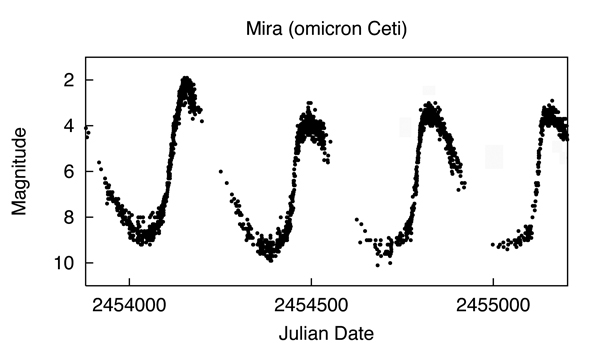
\includegraphics[width=\textwidth]{./img/CProblema/omicet.jpg}
    \caption{Curva de luz de una estrella Mira}
    \label{fig:gull}
  \end{subfigure}%
  ~ %add desired spacing between images, e. g. ~, \quad, \qquad, \hfill etc.
  % (or a blank line to force the subfigure onto a new line)
  \begin{subfigure}[b]{0.5\textwidth}
    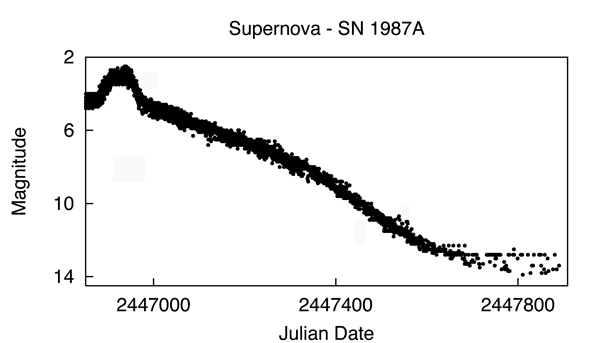
\includegraphics[width=\textwidth]{./img/CProblema/sn1987a.jpg}
    \caption{Curva de luz de la Supernova 1987A}
    \label{fig:tiger}
  \end{subfigure}
  ~ %add desired spacing between images, e. g. ~, \quad, \qquad, \hfill etc.
  % (or a blank line to force the subfigure onto a new line)
  \caption{Las estrellas pueden ser clasificadas en grupos basado en la forma de sus curvas de luz. Estas clasificación puede ser hecha con base en la forma de las curvas de luz, sin embargo es difícil crear un modelo matemático que capture estas diferencias. Imágenes tomadas de \cite{bsj_types_2012}}\label{fig:dosCurvas}
\end{figure} 

El reconocimiento de patrones es una disciplina científica cuya meta es la clasificación de objetos en clases. Existen situaciones en las cuales existe una gran cantidad de objetos previamente clasificados en clases predefinidas y la tarea es encontrar, o aproximar lo mejor posible, la dependencia funcional entre objetos y clases. Podemos precisar esto de la siguiente forma. Llamemos al espacio de los objetos que queremos clasificar $X$y $\{1,\dots, M\}$ es el conjunto de las posibles clases a las que pueden pertenecer los elementosd e $X$.  En el caso de la clasificación de curvas de luz, $X$ consta de todas las curvas de luz y  $\{1,\dots, M\}$ representa los posibles tipos de variabilidad estelar. Contamos con una muestra aleatoria de tamaño $N$, llamada muestra de entrenamiento, $\mathcal{L} = \{(x_i,j_i), \dots, (x_N,j_N)\}$  con $x_l\in X$ y $j_l\in \{1, \dots, M\}$, es decir, una muestra de $X$ previamente clasificada. Nuestra tarea es entonces proponer una función $g:X\rightarrow \{1,\dots, M\}$ a partir de la información contenida en $\mathcal{L}$ que representa nuestra predicción de la clase a la que pertenece cada elemento de $X$. La función $g$ se llama clasificador y, para un elemento $x\in X$ cuya clase $j$ es desconocida, el clasificador falla si $g(x)\neq j$.

El espacio $X$ puede ser complejo o no estar matemáticamente bien definido, por lo cual con frecuencia se representan los objetos con vectores, llamados de características,  en $\mathbb{R}^n$. Por ejemplo si queremos realizar detección de rostros, $X$ consiste de todos los posibles rostros, por lo que es más conveniente representar cada rostro con un conjunto de números como la separación de los ojos, el ángulo que forma las líneas que unen los ojos con la barbilla, etcétera; lo mismo sucede con las curvas de luz, por lo que representamos cada una con un vector. Estos vectores de características pueden, en principio, ser una combinación de variables continuas, discretas y categóricas, sin embargo esto no afecta en gran medida la teoría. Así las cosas, la elección de un clasificador puede ser una función $g:\mathbb{R}^n\rightarrow \{1, \dots, M\}$.

Se debe utilizar un marco probabilístico para modelar la dependencia entre características y clases. Puede suceder que dos observaciones con un mismo vector de características pertenezcan a clases diferentes. Esto puede suceder en escenarios en los que pertenencia a una u otra clase no so sea completamente explicada por diferencias en los vectores de características, o porque la dependencia real entre características y clases sea no determinista. En este orden de ideas suponemos que existe una medida de probabilidad $P$ sobre $\mathbb{R}^n\times \{1, \dots, M\}$ tal que $P(\vec{x}, j)$ es la probabilidad de observar un vector de características $\vec{x}\in\mathbb{R}^n$ cuyo objeto representado pertenece a clase $j$. Así definimos la probabilidad de error del clasificador $g$, $P_{e}(g)$, como 
\begin{equation}
P_e(g) = P(g(\vec{x})\neq j).
\end{equation}

Surge entonces la pregunta de qué tan bueno puede ser un clasificador. El mejor clasificador posible es llamado el clasificador de Bayes.

\section{El Clasificador de Bayes y Consistencia}

Decimos que un clasificador $g^*:\mathbb{R}^n\rightarrow \{1, \dots, M\}$ es de Bayes si minimiza la probabilidad de error, es decir, que si $g$ es otro clasificador entonces
\begin{equation}
P_e(g^*) \leq P_e(g).
\end{equation}
Llamaremos $P_{e}^{*}$ a  $P_e(g^*)$.

En el caso de que existan densidades condicionales $f_j$ tales que para cada $A\subset \mathbb{R}^n$ medible se cumple
\begin{equation}
P(A|j) =\int_{A}f_{j}(\vec{x})d\vec{x}
\end{equation}
podemos dar una expresión explícita para el clasificador de Bayes. Para un clasificador $g$ podemos escribir
\begin{equation}
  \begin{aligned}
    P_e(g) &= 1-P(g(\vec{x}) =  j)\\
    & = 1-\sum_{j=1}^{M} P(g(\vec{x}) = j|j)P(j)\\
    & = 1-\sum_{j=1}^{M}\left( \int_{\{g(\vec{x})=j\}}f_j(\vec{x})  d\vec{x} \right) P(j)\\
    & = 1 - \int \sum_{j=1}^{M} \chi_{\{g(\vec{x})=j\}}f_j(\vec{x})P(j)d\vec{x}.
  \end{aligned}
\end{equation}
Donde $P(j)$ es la probabilidad \textit{a priori} de encontrar un objeto de clase $j$ y $\chi_A$ es la función indicadora del conjunto $A$. Ahora, para cada $\vec{x}$ 
\begin{equation}\label{eq:bayesIneq}
\sum_{j=1}^{M}\chi_{\{g(\vec{x})=j\}}f_j(\vec{x})P(j) \leq \max_j[f_j(\vec{x})P(j)]
\end{equation}
entonces
\begin{equation}
P_e(g)\geq 1-\int \max_j[f_j(\vec{x})P(j)] d\vec{x}.
\end{equation}
Como la desigualdad \ref{eq:bayesIneq} es igualdad cuando $g$ le asigna a cada $\vec{x}$ la clase $j$ para la cual $f_j(\vec{x})P(j)$ es máximo, podemos concluir que éste es el clasificador de Bayes, es decir,
\begin{equation}\label{eq:clasificadorBayes}
  g^*(\vec{x}) = \argmax_{j\in\{1,\dots,M\}}f_j(\vec{x})P(j)
\end{equation}
y
\begin{equation}
  P_e^* = 1-\int \max_j[f_j(\vec{x})P(j)] d\vec{x}.
\end{equation}
$g^*$ es el estimador de máxima verosimilitud para $j$ y le asigna a cada $\vec{x}$ la clase que hace que la observación $\vec{x}$ sea más probable.

El hecho de que este clasificador sea el mejor posible nos muestra la importancia de elegir un vector de características de forma tal que las clases, es decir, sus distribuciones marginales $f_j$ se superpongan lo menos posible en el espacio de características. Aunque esto es intuitivamente obvio, esto nos da un argumento para afirmarlo. $f_j(\vec{x})P(j)$ puede ser interpretado como la probabilidad de que el vector $\vec{x}$ sea generado por la clase $j$. Si dos clases generan puntos en una región del espacio n-dimensional con probabilidad parecida, al clasificar un punto en esa región se esperará una probabilidad de error alta. En el caso extremo en que se le asigna a cada objeto un vector constante, el clasificador \ref{eq:clasificadorBayes} se reduce a escoger la clase que sea más probable \textit{a priori}.

En realidad rara vez se conocen las distribuciones marginales $f_j$ y frecuentemente no se conocen la probabilidades $P(j)$. Las probabilidades \textit{a priori} pueden ser dadas por el analísta o estimadas a partir de los datos si la muestra es representativa de $X$. Algunos métodos intentan estimar estas distribuciones marginales con funciones $\tilde{f}_j$ y utilizar el clasificador 
\begin{equation}
  g(\vec{x}) = \argmax_{j\in\{1,\dots,M\}}\tilde{f}_j(\vec{x})P(j)
\end{equation}
por ejemplo suponiendo alguna forma para las distribuciones $f_j$ o utilizando métodos no paramétricos de estimación de densidades como estimación por núcleos. La estimación de densidades por núcleos ha probado ser útil porque se sabe que el estimador $\tilde{f}_{j}$ de la densidad $f_j$ converge en media cuadrática, es decir,
\begin{equation}
  \int\left(f(\vec{x})-\tilde{f}(\vec{x})\right)^2d\vec{x}\rightarrow 0\text{ cuando } N\to\infty
\end{equation}
 sin embargo en dimensión $d$ se ha demostrado que estos convergen a una velocidad de $O(N^{1/(4+d)})$(REVISAR Y CITA) por lo cual no son prácticos en dimensiones altas. 

En la práctica, elegimos un clasificador entre una familia $\mathcal{H}$ de clasificadores posibles, llamados hipótesis, mediante un algorítmo de aprendizaje. Por ejemplo un árbol de clasificación y regresión es un árbol binario de decisón con funciones sencillas de decisión en cada nodo; existe un algorítmo para  escoger un árbol entre todos los árboles binarios posibles posibles. Una manera natural de elegir este clasificador es minimizar la probabilidad de error empírica
\begin{equation}
\hat{P}_{e}(g) = \frac{1}{N}\sum_{i=1}^{N}\chi_{\{g(\vec{x}_i)\neq j_{i}\}},
\end{equation}
es decir, elegir el clasificador
\begin{equation}\label{eq:empiricalErrorMin}
  g_{\mathcal{H}, N}^{*} = \argmin_{g\in\mathcal{H}} \hat{P}_{e}(g).
\end{equation} 
para el cual el error de clasificación es
\begin{equation}
  P_{\mathcal{H}, N}^{*} = \min_{g\in\mathcal{H}} \hat{P}_{e}(g).
\end{equation}

Se dice que un clasificador elegido con el criterio  \ref{eq:empiricalErrorMin} es consistente si $P_{\mathcal{H},N}^{*}\to P_e^*$ cuando $N\to\infty$.
Surge entonces la pregunta de bajo qué condiciones un clasificador es consistente. Es posible demostrar que las regla de decisión de k vecinos más cercanos \cite{devroye_probabilistic_1996}, bosques aleatorios \cite{biau_consistency_2008} y máquinas de soporte vectorial \cite{steinwart_consistency_2005} son constistentes. La idea utilizar la minimización del error empírico para elegir clasificadores fue desarrollada por Vapnik y Chervonenkis (citas están en p187 del Devroye, PONER). Para saber más, es posble consultar \cite{devroye_probabilistic_1996}.

En aplicaciones no se conoce la probabilidad mínima de error $P_e^*$ por lo que no es posible saber en términos absolutos qué tan bueno es un clasificador en un problema específico. Además de encontrar clasificadores que logren probabilidades tan bajas como sea posible, también es necesario implementar algorítmos de aprendizaje que sean eficientes y cuyos tiempos de ejecución no crezcan demasiado rápido con el tamaño de la muestra. Para juzgar un clasificador $g$ es necesario estimar la su probabilidad de error $P_e(g)$.

\section{Estimación del Error}

Uno de los métodos más populares para estimar la probabilidad de clasificación correcta de la función de decisión entrenada por un algorítmo de aprendizaje es validación cruzada de $v$ iteraciones. Se divide la muestra $\mathcal{L}$ en $v$ muestras de prueba $\mathcal{L}_{k}$, $k=1,\dots,v$ con el mismo número de elementos (o lo más próximo posible) y se define la $k$-ésima muestra de entrenamiento como $\mathcal{L}^{k} = \mathcal{L}\setminus \mathcal{L}_{k}$. Utilizando cada una de las $v$ muestras de entrenamiento $\mathcal{L}^{k}$  se puede entrenar una regla de decisión utilizando el algorítmo de aprendizaje en cuestión. Con ella se clasifican los elementos de la muestra de prueba $\mathcal{L}^{k}$ y se calcula $N_{ij}^{k}$ el número de elementos de de la clase $j$ clasificado como $i$. Sea $N_{ij}=\sum_{k}N_{ij}^{k}$ el número total de elmentos de la clase $j$ clasificado como $i$. Es posible estimar la probabilidad de que un elemento de la clase $j$ sea clasificado como $i$, $P^{VC}(g(\vec{x})=i|j)$, con $N_{ij}/N_{j}$, donde $N_{j}$ es el número de elementos pretenecientes a la clase $j$ en la muestra $\mathcal{L}$. Intuitivamente, si la muestra es grande tendremos aproximadamente el mismo poder para clasificar con la muestra completa que con una fracción $\frac{v-1}{v}$ de ella, por lo cual $P^{VC}$ será una buena aproximación a la probabilidad real de clasificación. El valor $v = 10$ es popular en la literatura aunque esta elección es un poco arbitraria. Una elección de $v$ grande da estiamdos menos pesimistas de la probabildiad de error, sin embargo aumentar $v$ aumenta el costo computacional del estimado, por lo que estos dos apectos deben ser balanceados.

A continuación exponemos algunos clasificadores.

\section{Clasificadores}

\subsection{k Vecinos Más Cercanos}

K vecinos más cercanos (knn por sus iniciales en inglés) fue propuesto por Fix y Hodges en \cite{fix_discriminatory_1951}, y luego republicado en  \cite{silverman_e._1989}. Se basa en el principio de que los ejemplos de una misma clase se encuentran cerca y que es posible clasificar uno basado en la observación de la clase de sus vecinos más cercanos\footnote{Dime con quién andas y te diré quién eres}. Dado un entero $k$ fijo, esta regla le asigna a cada punto de $\mathbb{R}^n$ la clase a la que pertencen la mayoría de los $k$ elementos más cercanos a $\vec{x}$ entre los elementos de la muestra $\{\vec{x}_1, \dots,\vec{x}_N\}$, esto es,
\begin{equation}\label{eq:knnRule}
 g^{knn}(x) = j  \text{ tal que } \sum_{i=1}^{N}w_{i,N}\chi_{\{j_i = j\}} > \sum_{i=1}^{N}w_{i,N}\chi_{\{j_i = k\}}\forall k\neq j
\end{equation} 
donde $w_{i,N} = 1/k$ si $\vec{x}_i$ está entre los $k$ vecinos más cercanos de $\vec{x}$ y es $0$ de lo contrario. $w_{i,N}$ es llamado peso. Es posible demostrar que knn es consistente en el caso en que $k/N\to 0$ cuando $N\to \infty$ para cualquier elección de pesos $w_{i,N}$ siempre y cuando no permita la clasificación en una clase con minoría numérica \cite{devroye_probabilistic_1996}.

En primera aproximación, se puede implementar un algorítmo que clasifica un punto $\vec{x}$ en un tiempo $O(Nk)$, sin embargo es posible crear estructuras de datos que hacen esta búsqueda más eficiente. Por ejemplo un COVER TREE (traducir)\cite{beygelzimer_cover_2006} es una estructura de datos que ocupa $O(N)$ espacio, puede ser construida en un tiempo de $O(N\log{N})$ y permite realizar búsquedas en tiempo $O(\log{N})$ y ha mostrado aumentar la velocidad de las búsquedas entre uno y varios órdenes de magnitud con respecto a utilizar el algorítmo de fuerza bruta (Beygelzimer). Esta estructura se encuentra implementada en el paquete FNN (cite) para R.

Existen algunas variaciones de knn como knn empaquetado\footnote{En inglés \textit{bagged knn}. \textit{Bagging} es una abreviación de \textit{bootstrap aggregating}.} \cite{breiman_heuristics_1996, breiman_bagging_1996} y esquemas de pesos óptimos \cite{samworth_optimal_2012}. El proceso de empaquetado fue propuesto por \cite{breiman_heuristics_1996, breiman_bagging_1996} y consiste en que, dado un punto $\vec{x}$, este es clasificado usando la regla de la mayoría entre $n$ clasificadores de knn que utilizan submuestras de tamaño $m<N$ tomadas de la muestra original con reemplazo. Este procedimiento ha mostrado aumentar la precisión de los clasificadores \cite{breiman_bagging_1996}. Por otra parte, puede demostrarse que la elección de pesos dada en la ecuación \ref{eq:knnRule} es asintóticamente óptima, sin embargo hay situaciones en las que una elección de pesos puede mejorar la precisión. Por ejemplo \cite{samworth_optimal_2012} dio pesos óptimos para el caso en que la dimensión de los datos es 4. 

\subsection{Máquinas de Soporte Vectorial}

%%Introducción
Las Máquinas de Soporte Vectorial (MSV) son sistemas de clasificación que utilizan con conjunto de hipótesis las funciones lineales en un espacio de dimensión alta. Las MSV como se conocen hoy en día fueron propuestas por Cortes y Vapnik en \cite{cortes_support-vector_1995} basado en utilizar núcleos para para encontrar un plano que maximice la distancia a los puntos de la muestra, o equivalentemente, de margen maximal. Daremos una discusión sobre clasificadores lineales y clasificadores lineales de margen maximal, luego mencionamos los conceptos de optimización convexa que son la base de la utilización de núcleos para MSV y finalmente referenciamos el algorítmo de Minimización Secuencial Óptima. Seguimos el texto de Cristianini y Shawe-Taylor \cite{cristianini_introduction_2000} en el que se puede encontrar una introducción completa a MSV y la teoría de optimización convexa necesaria para MSV. Para consultas sobre temas adicionales sobre optimización convexa, se puede consultar el libro de Boyd, Vandenberghe y Lieven \cite{boyd_convex_2004}.

%Introducción a los clasificadores lineales%
Las MSV son clasificadores binarios, es decir, solo pueden distinguir entre dos clases. Para casos en los que se necesita clasificar más de dos clases, es posible implementar esquemas de votación que serán expuestos más adelante. Primero describimos los clasificadores lineales en $\mathbb{R}^n$ en casos en los que se puede escoger un plano que separe perfectamente las dos clases y luego extendemos estos métodos para casos en lo que esto no es posible. Supongamos que se tiene un problema de clasificación binario donde el conjunto de las clases bosibles es $\{-1,1\}$. Consideremos clasificadores lineales de la forma
\begin{equation}\label{eq:clasificadorLineal}
g(\vec{x}) = signo( \langle \vec{w}, \vec{x} \rangle + b).
\end{equation}
 Una muestra de entrenamiento de tamaño N  $\mathcal{L} = \{(\vec{x}_1, j_1), \dots, (\vec{x}_N, j_N)\}$ es linealmente separable si existe un plano definido por $\langle \vec{w}, \vec{x} \rangle +b =0$ tal que
\begin{equation}\label{eq:linSep}
j_{i}\left(\langle \vec{w}, \vec{x}_i \rangle +b\right)> 0, i = 1,\dots, N.
\end{equation}
Nos referiremos al plano $\langle \vec{w}, \vec{x} \rangle +b = 0$ con la notación abreviada $(\vec{w},b)$. $\vec{w}$ es el vector perpendicular al plano y la condición \ref{eq:linSep} corresponde a que los elementos de la clase $1$ quedan ubicados en el semiespacio definido por $\langle \vec{w}, \vec{x} \rangle +b > 0$, mientras que los pertenecientes a la clase $-1$ quedan en el semiespacio $\langle \vec{w}, \vec{x} \rangle + b< 0$. Este plano puede no estar bien definido, en el sentido de que puede haber más de un plano separador para un conjunto de datos, por lo que es necessario definir una noción de lo que significa elegir ``el mejor'' plano.

Podemos elegir el plano maximizando la distancia entre el plano y los ejemplos, por lo que es necesario definir la noción de margen. Definimos el margen funcional $\gamma_i$ de un ejemplo $(\vec{x}_i, j_i)$ con respecto al hiperplano $(\vec{w}, b)$ como
\begin{equation}
\gamma_i = j_i(\langle\vec{w}, \vec{x}_i \rangle + b).
\end{equation}
Un ejemplo $(\vec{x}_i, j_i)$ es clasificado de manera correcta por el plano $(\vec{w}, b)$ si $\gamma_i>0$ y nos referimos al  mínimo de los márgenes funcionales de la muestra como el margen funcional de un plano. También podemos tomar el margen con respecto plano normalizado $(\frac{\vec{w}}{\|\vec{w}\|},\frac{b}{\|\vec{w}\|})$ en cuyo caso el margen funcional mide la distancia euclidiana entre el punto $\vec{x}_i$ y el plano. En esta situación nos referiremos al margen como  margen geométrico. 

Como $(\lambda\vec{w}, \lambda b)$ define el mismo plano que $(\vec{w}, b)$  para todo $\lambda \neq 0$, tenemos un grado de libertad para elegir el plano separador. Podemos llevar a cabo un truco para expresar el margen funcional del plano en términos de la norma de $\vec{w}$ y así traducir el problema de encontrar el plano a un problema de optimización. Por tener un grado de libertad,  podemos maximizar el margen geométrico manteniende el margen funcional fijo e igual a 1. En este caso, si $\vec{w}$ es el vector que alcanza un margen funcional de 1 en el punto  positivo$\vec{x}^+$ y $-1$ en el punto negativo $\vec{x}^-$, podemos calcular su margen geométrico de la siguiente forma. Como tener un margen funcional de $\pm 1$ significa que $\langle \vec{w}, \vec{x}^{\pm}\rangle +b = \pm 1$ tenemos que el margen geométrico $\gamma$ del plano cumple
\begin{equation}
  \begin{aligned}
    \gamma &=\frac{1}{2}\left(\left\langle\frac{\vec{w}}{\|\vec{w}\|},\vec{x}^+\right\rangle-\left\langle\frac{\vec{w}}{\|\vec{w}\|},\vec{x}^-\right\rangle\right) \\
    & = \frac{1}{\|\vec{w}\|}\\ 
  \end{aligned}
\end{equation}
por lo que encontrar el plano que maximize el margen geométrico es equivalente a solucionar el problema de optimización
\begin{equation}\label{eq:optimizacionLinSep}
\begin{aligned}
& \underset{\vec{w},b}{\text{minimizar}}
& & \langle \vec{w}, \vec{w} \rangle \\
& \text{sujeto a}
& & j_i(\langle \vec{w}, \vec{x_i}\rangle + b)\geq 1, \; i = 1, \ldots, N,
\end{aligned}
\end{equation}
donde la restricción hace que el margen funcional de cada $\vec{x}_i$ con respecto al plano sea mayor o igual que 1, porque elegimos el plano con margen 1. Así, podemos traducir el problema de encontrar el plano separador para una muestra linealmente separable con el problema de optimización convexa \ref{eq:optimizacionLinSep}.

Hasta ahora solo hemos consierado situaciones en las que los datos $(\vec{x}_i,j_i)$ son linealmente separables. Para permitir clasificaciones erróneas podemos introducir variables de holgura $\xi_i>0$ en el problema de optimización \ref{eq:optimizacionLinSep} para que los algunos ejemplos puedan ser clasificados erróneamente, es decir,  $j_i(\langle \vec{w}, \vec{x_i}\rangle + b)\geq 1-\xi_i$. También debemos introducir un costo asociado al vector de holgura $\vec{\xi}=(\xi_1,\dots,\xi_N)$, por lo que la función objetivo será una combinación del costo y la función objetivo original. En el caso en que se utilice la norma 1 del vector $\vec{\xi}$, el problema de optimización \ref{eq:optimizacionLinSep} se convierte en 
\begin{equation}
  \begin{aligned}
    & \underset{\vec{w},b, \vec{\xi}}{\text{minimizar}}
    & & \langle \vec{w}, \vec{w} \rangle +C\sum_i\xi_i,\\
    & \text{sujeto a}
    & & j_i(\langle \vec{w}, \vec{x_i}\rangle + b)\geq 1-\xi_i, \\
    & & & \xi_i>0, \\
    & & & i = 1, \ldots, N,
  \end{aligned}
\end{equation}
y al elegir la norma 2
\begin{equation}
  \begin{aligned}
    & \underset{\vec{w},b, \vec{\xi}}{\text{minimizar}}
    & & \langle \vec{w}, \vec{w} \rangle +C\sum_i\xi_i^2,\\
    & \text{sujeto a}
    & & j_i(\langle \vec{w}, \vec{x_i}\rangle + b)\geq 1-\xi_i, \\
    & & & \xi_i>0, \\
    & & & i = 1, \ldots, N,
  \end{aligned}
\end{equation}
que es equivalente al mismo problema tras eliminar la restricción $\xi_i>0$, esto es,
\begin{equation}\label{eq:problemaOptimizacionPrimalMSV}
  \begin{aligned}
    & \underset{\vec{w},b, \vec{\xi}}{\text{minimizar}}
    & & \langle \vec{w}, \vec{w} \rangle +C\sum_i\xi_i^2,\\
    & \text{sujeto a}
    & & j_i(\langle \vec{w}, \vec{x_i}\rangle + b)\geq 1-\xi_i, \\
    & & & i = 1, \ldots, N,
  \end{aligned}
\end{equation}
donde $C$ es un número que debe ser calibrado, utilizando estimaciones del error como validación cruzada. Elegimos la norma 2 como costo porque se pueden dar cotas para el errror de generalización, esto es, el error cometido al clasificar ejemplos que no están incluídos en la muestra de aprendizaje, basadas en la norma 2 del vector de holgura $\vec{\xi}$ (ver \cite{cristianini_introduction_2000}), por lo que minimizar la norma 2 implica disminuir el error de generalización. El problema de optimización \ref{eq:optimizacionLinSep} es también un problema de optimización convexa.

La observación clave para la construcción del método de MSV es observar que el problema dual de \ref{eq:problemaOptimizacionPrimalMSV} solo depende de el ptoducto interno entre los datos $\vec{x}_i, i = 1,\dots,N$. Para ello es necesario definir el lagrangiano y el problema dual de un problema de optimización. Adicionalmente damos lasa condiciones de Karush-Kuhn-Tucker, que tienen como consecuencia el fenómeno que le da el nombre a MSV. Recordemos que para un  problema de optimización de la forma 
\begin{equation}\label{eq:problemaDeOptimizacionGeneral}
  \begin{aligned}
    & \underset{\vec{w}\in\mathcal{D}}{\text{minimizar}}
    & & f_0(\vec{w})\\
    & \text{sujeto a}
    & & f_i(\vec{w}) \leq 0 , i = 1,\dots,m,\\
    & & & h_i(\vec{w}) = 0, i = 1, \dots, p,
  \end{aligned}
\end{equation}
podemos definir su lagrangiano 
\begin{equation}
  L(\vec{w}, \vec{\alpha}, \vec{\beta}) = f_0(\vec{w}) + \sum_{i=1}^{m}\alpha_if_i(\vec{w}) + \sum_{i=1}^{p}\beta_ih_i(\vec{w})
\end{equation}
y su función dual 
\begin{equation}
  W(\vec{\alpha}, \vec{\beta}) = \inf_{\vec{w}\in\mathcal{D}}L(\vec{w}, \vec{\alpha}, \vec{\beta})
\end{equation}
para la cual se cumple
\begin{equation}
  W(\vec{\alpha}, \vec{\beta}) \leq L(\vec{w}, \vec{\alpha}, \vec{\beta}) \leq f_0(\vec{w})
\end{equation}
siempre que $\alpha_i\geq 0, i = 1,\dots, m$. Como $g$ es una cota inferior para $f_0$, podemos preguntar si maximizar $g$ y minimizar $f_0$ son problemas equivalentes. Por lo anterior consideramos el problema dual de optimización
\begin{equation}\label{eq:problemaOptimizacionDualGeneral}
  \begin{aligned}
    & \underset{\vec{\alpha},\vec{\beta}}{\text{maximizar}}
    & & W(\vec{\alpha}, \vec{\beta})\\
    & \text{sujeto a}
    & & \alpha_i \geq 0 , i = 1,\dots,m.
  \end{aligned}
\end{equation}
En general no se tiene que maximizar $W$ y minimizar $f_0$ sean problemas equivalentes. En el caso de que sí lo sean se dice que se hay dualidad fuerte. Sin embargo, es posible probar que, para el caso en el que estamos interesandos, en el que el problema es de la forma \ref{eq:problemaDeOptimizacionGeneral} con $\mathcal{D}$ un dominio convexo\footnote{Un conjunto $\mathcal{D} \subseteq \mathbb{R}^n$ es convexo si para todos $d_1, d_2\in\mathcal{D}$ se cumple $\theta d_1+(1-\theta)d_2\in\mathcal{D}$}, $f_0$ convexa\footnote{Una función $f(\vec{w})$ es convexa si $f(\theta\vec{w}_{1}+(1-\theta)\vec{w}_{2})\leq \theta f(\vec{x}_{1})+(1-\theta)f(\vec{x}_{2})$ para cada $\theta\in[0,1]$} y $f_1,\dots,f_m,h_0,\dots,h_p$ funciones afines\footnote{Una función $h(\vec{w})$ es afín si es de la forma $h(\vec{w}) = A\vec{w}+\vec{v}$, las funciones afines son convexas} entonces hay dualidad fuerte.

Si el problema de optimización \ref{eq:problemaDeOptimizacionGeneral} es convexo, es decir, si $f_0,\dots, f_m$ son funciones convexas y $h_0,\dots,h_p$ son afines, en el caso de que $f_0,\dots, f_m$ son diferenciables es posible demostrar que para que $\vec{w}^*$ sea el punto óptimo de problema \ref{eq:problemaDeOptimizacionGeneral} es necesario y suficiente que exista $(\vec{\alpha}^*,\vec{\beta}^*)$ que cumplan las condiciones de Karush-Kuhn-Tucker (KKT)

\begin{align}
    f_i(\vec{w}^*) &\leq 0, & i=1,\dots,m, \\
    h_i(\vec{w}^*) &= 0, & i=1,\dots,p, \\
    \alpha_i^* &\geq 0, & i=1,\dots,m, \\
    \alpha_i^*f_i(\vec{w}^*) & = 0, & i=1,\dots,m, \label{eq:condicionComplementariedad}\\
    \nabla f_0(\vec{w}^*) + \sum_{i=1}^{m}\alpha_i^*\nabla f_i(\vec{w}^*) + \sum_{i=1}^{p}\beta_i^*\nabla h_i(\vec{w}^*) & = 0. &
\end{align}

Ahora retomamos el problema original. El lagrangiano del problema \ref{eq:problemaOptimizacionPrimalMSV} es 
\begin{equation}
  L(\vec{w},b,\vec{\xi},\vec{\alpha}) = \frac{1}{2}\langle \vec{w}, \vec{w} \rangle + \frac{C}{2}\sum_{i}^{N}\xi_i^2 + \sum_{i=1}^{N}\alpha_i\left[\gamma_i(\langle \vec{w}, \vec{x}_i \rangle +b) -1 + \xi \right].
\end{equation}
Para calcular la función dual $W$ calculamos los puntos críticos de $L$
\begin{align}
    \frac{\partial L}{\partial\vec{w}} & = \vec{w} - \sum_{i=1}^{N}j_i\alpha_i\vec{x}_i = \vec{0}\label{eq:vectorPesoEnVarsDuales}\\
    \frac{\partial L}{\partial\vec{\xi}} & = C\vec{\xi}-\vec{\alpha} = \vec{0}\label{eq:alphaYXi}\\
    \frac{\partial L}{\partial b} & = \sum_{i=1}^{N}j_i\alpha_i = 0
\end{align}
con lo que obtenemos 
\begin{equation}
W(\vec{\alpha}) = \sum_{i=1}^N \alpha_i -\frac{1}{2}\sum_{i,k=1}^Nj_ij_k\alpha_i\alpha_k\left( \langle\vec{x}_i, \vec{x}_k\rangle + \frac{1}{C}\delta_{ik}  \right).
\end{equation}
por lo que lo que el problema de optimización \ref{eq:problemaOptimizacionPrimalMSV} es equivalente (por haber dualidad fuerte) al problema de optimización
\begin{equation}\label{eq:problemaOptimizacionDualMSV}
  \begin{aligned}
    & \underset{\vec{\alpha}}{\text{maximizar}}
    & & \sum_{i=1}^N \alpha_i -\frac{1}{2}\sum_{i,k=1}^Nj_ij_k\alpha_i\alpha_k\left( \langle\vec{x}_i, \vec{x}_k\rangle + \frac{1}{C}\delta_{ik}  \right)\\
    & \text{sujeto a}
    & & \sum_{i=1}^Nj_i\alpha_i = 0, \\
    & & & \alpha_i \geq 0, i = 1,\dots,N,
  \end{aligned}
\end{equation}
donde $\delta_{ik}$ es la función delta de Kronecker, $\delta_{ik} = 1$ si $i=k$ y $0$ de lo contrario. Si $\alpha^*$ es la solución al problema \ref{eq:problemaOptimizacionDualMSV}, las condiciones \ref{eq:condicionComplementariedad}, llamadas condiciones de complementariedad, que son en este caso 
\begin{equation}\label{eq:condicionComplementariedadMSV}
\alpha_{i}^{*}[j_i(\langle\vec{w},\vec{x}_i\rangle+b)-1+\xi_i] = 0
\end{equation}
nos muestran que para los $\vec{x}_i$ que se encuentran en el margen o mal clasificados $\alpha_i\neq 0$ y de lo contrario $\alpha_i = 0$. Los vectores para los cuales $\alpha_i\neq 0$ son llamados vectores de soporte porque el plano encontrado está únicamente determinado por ellos. Por esto, se dice que la solución es dispersa. Esto se puede ver en la ecuación \ref{eq:vectorPesoEnVarsDuales}, que muestra que los vectores de soporte son los únicos que aportan al vector $\vec{w}$ que define el plano, esto es, 
\begin{equation}
\vec{w} = \sum_{i=1}^{N}j_i\alpha_i^*\vec{x}_i = \sum_{i\in vs}j_i\alpha_i^*\vec{x}_i
\end{equation}
donde $i\in vs$ hace referencia a los $\vec{x}_i$ que son vectores de soporte. $b$ es escogido de tal manera que para los vectores de soporte su cumpla  
\begin{equation}\label{eq:eleccionb}
  j_i(\langle\vec{w},\vec{x}_i\rangle+b) = 1-\xi_i = 1-\frac{\alpha_i^*}{C}, i\in vs
\end{equation}
por las equaciones \ref{eq:condicionComplementariedadMSV} y \ref{eq:alphaYXi}. Con lo anterior el clasificador \ref{eq:clasificadorLineal} encontrado al solucionar el problema de optimización es 
\begin{equation}\label{eq:clasificadorMargenMaximal}
g(\vec{x}) = signo\left(\sum_{i\in vs}j_i\alpha^*_i\langle\vec{x}_i,\vec{x}\rangle + b \right)
\end{equation}
cuyo margen geométrico $\gamma = \frac{1}{\| \vec{w} \|}$ se puede calcular con
\begin{equation}
  \begin{aligned}
    \langle\vec{w},\vec{w}\rangle &= \sum_{i,k\in vs}j_ij_k\alpha_i\alpha_k\langle\vec{x}_i,\vec{x}_k\rangle\\
    &= \sum_{i\in vs}j_i\alpha_i\sum_{k\in vs}j_k\alpha_k\langle\vec{x}_i,\vec{x}_k\rangle\\
    &= \sum_{i\in vs}\alpha_{i}^{*}(1-\xi_i^*-j_ib^*)\\
    &=  \sum_{i\in vs}\alpha_i^*-\sum_{i\in vs}\alpha^*_i\xi_i^*\\
    &= \sum_{i\in vs}\alpha_i^*-\frac{1}{C}\langle\vec{\alpha}^*,\vec{\alpha}^*\rangle
  \end{aligned}
\end{equation} 
por lo cual 
\begin{equation}\label{eq:margenGeometrico}
\gamma = \left(\sum_{i\in vs}\alpha_i^*-\frac{1}{C}\langle\vec{\alpha}^*,\vec{\alpha}^*\rangle\right)^{-1/2}.
\end{equation}

Ahora tenemos todos los ingredientes encesarios para introducir el uso de núcleos para MSV. La observación central de MSV es que el problema de optimización \ref{eq:problemaOptimizacionDualMSV} solo depende de los datos $\vec{x}_1,\dots,\vec{x}_N$ a través de la matriz $\left( \langle\vec{x}_i, \vec{x}_k\rangle \right)_{i,k=1}^N$, llamada matriz de Gram. Si podemos calcular la matriz de Gram para una representación de los datos en un espacio con producto interno de dimensión mayor, podemos modificar el problema de optimización \ref{eq:problemaOptimizacionPrimalMSV} para encontrar un plano separador en ese espacio. Sea $\mathcal{H}$ un espacio de Hilbert con producto interno $\langle,\rangle_\mathcal{H}$, y $\phi:\mathbb{R}^n\to\mathcal{H}$ una función. Si logramos encontrar una función $K':\mathbb{R}^n\times\mathbb{R}^n\to\mathbb{R}$ tal que $K'(\vec{x},\vec{y}) = \langle\phi(\vec{x}),\phi(\vec{y})\rangle_{\mathcal{H}}$ podemos resolver el problema de optimización equivalente a \ref{eq:problemaOptimizacionDualMSV} para encontrar el plano de margen maximal en $\mathcal{H}$ usando una representación de los datos en $\mathcal{H}$ a través de $\phi$, es decir, resolver
\begin{equation}\label{eq:problemaOptimizacionDualKernelMSV}
  \begin{aligned}
    & \underset{\vec{\alpha}}{\text{maximizar}}
    & & \sum_{i=1}^N \alpha_i -\frac{1}{2}\sum_{i,k=1}^Nj_ij_k\alpha_i\alpha_k K\left(\vec{x}_i, \vec{x}_k\right)\\
    & \text{sujeto a}
    & & \sum_{i=1}^Nj_i\alpha_i = 0, \\
    & & & \alpha_i \geq 0 , i = 1,\dots,n. 
  \end{aligned}
\end{equation}
con $K(\vec{x},\vec{y}) = K'(\vec{x},\vec{y}) + \frac{1}{C}\delta(\vec{x},\vec{y})$, siendo $\delta$ la función delta de Dirac, $\delta(\vec{x},\vec{y}) = 1$ si $\vec{x}=\vec{y}$ y $\delta(\vec{x},\vec{y})= 0$ de lo contrario. En analogía con \ref{eq:clasificadorMargenMaximal}, el clasificador obtenido al resolver el problema de optimización \ref{eq:problemaOptimizacionDualKernelMSV} es 
\begin{equation}\label{eq:clasificadorMargenMaximalKernel}
g(\vec{x}) = signo\left(\sum_{i=1}^{N}j_i\alpha_i^*K\left(\vec{x}_i,\vec{x}\right) + b \right)
\end{equation}
con $b$ elegido como en \ref{eq:eleccionb} y margen geométrico \ref{eq:margenGeometrico}.

Existe un teorema, debido a Mercer \cite{mercer_functions_1909}, que da las condiciones necesarias para que $K(\vec{x},\vec{y}) = \langle\phi(\vec{x}),\phi(\vec{y})\rangle_{\mathcal{H}}$ para algún $\phi$, lo cual es computacionalmente eficiente puesto que evita la necesidad de conocer explícitamente el espacio $\mathcal{H}$ y la función $\phi$. Tal función $K$ es llamada núcleo. Para que $K(\vec{x},\vec{y})$ defina un producto interno es claro que debe ser definida positiva y simétrica. En el caso de dimensión finita, si $K$ es una matriz simétrica semidefinida positiva, entonces podemos escribir $K$ de la forma
\begin{equation}
 K =\sum_i\lambda_i v_iv_i^T
\end{equation}
por lo que, si escribimos $\vec{x} = (x_1,\dots,x_n)$ y $\vec{y}=(y_1,\dots,y_n)$ en la base normalizada de autovectores de $K$, $K$ define un producto interno $\langle\cdot,\cdot\rangle_{K}$ dado por
\begin{equation}
 K(\vec{x},\vec{y}) =x^TKy = \sum_{i,j}\lambda_ix^Tv_iv_i^Ty = \sum_i \lambda_ix_iy_i = \langle x,y\rangle_{K}
\end{equation}
siendo $\vec{v}_i$ los autovectores de $K$ y $\lambda_i\geq 0$ sus autovalores. Análogamente, si $\lambda_i$ y $\phi_i$ $i = 1,2,\dots$ son los autovalores y las autofunciones normalizadas del problema
\begin{equation}
  \int K(\vec{x},\vec{z})\phi(\vec{z})d\vec{z} = \lambda\phi(\vec{x}), 
\end{equation}
el teorema de Mercer da condiciones para que podamos escribir 
\begin{equation}
  K(\vec{x},\vec{z}) = \sum_{i=1}^{\infty}\lambda_i\phi_i(\vec{x})\phi_i(\vec{z}) =  \langle \phi(\vec{x}), \phi(\vec{y})\rangle_{\mathcal{H}}
\end{equation}
para $\phi(\vec{x}) = (\phi_1(\vec{x}), \phi_2(\vec{x}),\dots)$ y el producto interno definido por $\langle \psi,\varphi \rangle_{\mathcal{H}} = \sum_{i=1}^{\infty}\lambda_i\psi_i\varphi_i$. Sin ir en más detalle en el análisis, citamos el teorema.
%Teorema de Mercer
\begin{theorem}[Mercer]
  Sea $X$ un subconjunto compacto de $\mathbb{R}^n$. Suponga que $K$ es una función simétrica y continua tal que el operador integral $T_K:L_2(X)\to L_2(X)$
  \begin{equation*}
    (T_Kf)(\cdot)=\int_{X}K(\cdot,\vec{x})f(\vec{x})d\vec{x}
  \end{equation*}
  es positivo, esto es,
  \begin{equation*}
    \int_{X\times X}K(\vec{x},\vec{z})f(\vec{x})f(\vec{x})d\vec{x}d\vec{z}\geq 0
  \end{equation*} 
  para todo $f\in L_2(X)$. Entonces podemos expandir $K(\vec{x},\vec{z})$ en una serie iniformemente convergente en $X\times X$ en términos de las autofunciones $\phi_i\in L_2(X)$, nor malizadas de tal forma que $\|\phi_i\|_{L_2}=1$ y autovalores positivos $\lambda_i\geq 0$
  \begin{equation*}
    K(\vec{x},\vec{z}) = \sum_{i=1}^{\infty}\lambda_i\phi_i(\vec{x})\phi_i(\vec{z}).
  \end{equation*}
\end{theorem}

Con las condiciones anteriores, podemos encontrar el núcleo $K$, para encontrar el plano de margen maximal en el $\mathcal{H}$ resolviendo el problema de optimización \ref{eq:problemaOptimizacionDualKernelMSV} sin siquiera conocer explícitamente la función de representación $\phi$ ni $\mathcal{H}$. Si $K_1$, y $K_2$ son núcleos es posible demostrar que cualquier núcleo definifo por un polinomio de dos variables $K(\vec{x},\vec{z}) = p(K_1(\vec{x},\vec{z}),K_2(\vec{x},\vec{z}))$ también es un núcleo, así como $K(\vec{x},\vec{z})=\exp{(K_1(\vec{x},\vec{z}))}$. Un núcleo popular es el núcleo radial
\begin{equation}
K(x,y) = e^{-\gamma\|\vec{x}-\vec{y}\|^2},
\end{equation}
 que ha sido utilizado en gran variedad de aplicaciones \cite{cristianini_introduction_2000}. Al utilizar el núcleo radial se debe calibrar tanto como el costo $C$ y el ancho del núcleo $\gamma$ para minimizar la tasa clasificación errónea utilizando, por ejemplo, validación cruzada.

En el caso de clasificación en $M>2$ categorías se pueden implementar esquemas de votación. Una posible aproximación, llamada uno-contra-uno\footnote{En inglés \textit{one-against-one}}, es entrenar  $\frac{M(M-1)}{2}$ clasificadores que discriminen entre cada par de clases. Se escoge entonces la clase que haya sido decidida por la mayoría de clasificadores y en caso de empate se elige la que tenga índice menor. Otra aproximación, llamada uno-contra-resto\footnote{En inglés \textit{one-against-rest}} es entrenar $M$ clasificadores que discriminen entre cada clase y su complemento. Se elige la clase en que de la clasificación con el mayor margen.

El problema \ref{eq:problemaOptimizacionDualKernelMSV} es un problema de optimización convexa. Estos problemas han sido estudiados extensamente y existen formas eficientes de encontrar las soluciones que pueden ser aplicadas directamente. El principal obstáculo para utilizar estas aproximaciones es que el espacio necesario para almacenar la  matriz de Gram del problema crece cuadráticamente con el tamaño de la muestra dado que, en general, no es una matriz dispersa. Sin embargo se pueden explotar algunas características del problema, como el hecho de que la solución es dispersa para crear algorítmos eficientes. 

Optimización Secuencial Minimal (OSM) es un algorítmo utilizado para resolver el problema de optimización \ref{eq:problemaOptimizacionDualKernelMSV}. Se basa en el el requerimiento de que $\sum_i\alpha_ij_i = 0$ en todas las iteraciones del algorítmo, por lo que se deben actualizar a lo sumo dos $\alpha_i$ en cada paso. En cada paso OSM utiliza eurísticas para eligir dos $\alpha_i, \alpha_k$ para optimizar y utiliza el hecho de que este subproblema puede ser resuelto analíticamente, lo que elimina la necesidad de realizar operaciones con matrices. Este algorítmo logra reducciones en el tiempo de ejecución de varios órdenes de magnitud con respecto a algorítmos como el del gradiente. Existen implementaciones disponibles, como la librería libsvm escrita en C++ por Chih-Chung Chang and Chih-Jen Lin (cita libsvm) para la cual existe una interfaz para R en el paquete e1071 (cita e1071). Para clasificación en múltiples clases, libsvm utiliza el esquema de votación uno-contra-uno porque, basado en el análisis de (comparison, chin-wei) los resultados con ambas aproximaciones son comparables y el método uno-contra-uno toma menos tiempo de entrenamiento.

\subsection{Árboles de Clasificación y Regresión}

Árboles de Clasificación y Regresión (CART, por sus siglas en inglés) es un método de clasificación que utiliza el conjunto de los árboles de decisión binarios como conjunto de hipótesis. Este método fue propuesto por Breiman, Friedman, Olshen y Stone a lo largo de varios trabajos, que luego fueron condesados en \cite{breiman_classification_1984}. La metodología consiste en construir a partir de la muestra de entrenamiento árboles de decisión que a cada nodo terminal le asignan una clase, que es el resultado de la clasificación. Explicaremos la forma en que se construyen estos árboles. Una implementación libre se encuentra en el paquete rpart (cita rpart) para R.

El proceso de construcción de la regla de decisión consiste de dos pasos: primero construir un árbol lo suficientemente grande y luego podarlo para obtener un árbol con buenas propiedades de generalización. Inicialmente se cuenta con toda la muestra de aprendizaje; la muestra se divide en dos grupos utilizando un criterio de impureza (que será definido más adelante) en un grupo que pertenece a un subconjunto del espacio de características y otro que no. Nos referimos a estas divisiones como preguntas. Se hacen nuevas preguntas hasta que no se pueda mejorar  la pureza de las divisiones o hasta que cada nodo tenga un número mínimo de datos. Las divisiones de los datos pueden ser representadas con un árbol binario, lo que brinda una interpretación sencilla del clasificador. Subsecuentemente se poda el arbol resultante porque con frecuencia este es muy complejo y se sobreajusta a la muestra de aprendizaje. Una observación sin clasificar puede ser asignada  a uno de los nodos terminales del árbol utilizando las preguntas que resultaron de la construcción del arbol y se le asiga la clase que minimice el costo de clasificación estimado con la muestra de entrenamiento.  

Las divisiones hechas en cada nodo son preguntas hechas sobre una variable y para construir un arbol de decisión  de manera algorítmica se necesita un conjunto de pregutas predeterminadas. Por esta razón se necesita que la muestra tenga una estructura estándar. Una muestra de aprendisaje $\mathcal{L} = \{(\vec{x}_1,j_1),\dots,(\vec{x}_M,j_M)\}$ tiene estructura estándar si todos los vectores de características $\vec{x}$ tienen la forma $\vec{x} = (x_{1},\dots,x_{n})$ , es decir, tienen dimensionalidad fija y los $x_i$ están ordenados de tal forma que corresponden a la misma característica. Cada vector de características puede consistir de variables continuas o categóricas. En cada nodo se hace una pregunta y las preguntas estándar son de la forma $x_k\leq c$ en el caso de que $x_k$ sea continua y $x_m\in S$ en el caso que $x_m$ sea categórica, donde $S$ es un subconjunto de los posibles valores que la variable $x_m$ puede tomar. Las preguntas posibles pueden hacerse más complejas para incluír combinaciones lineales de características contínuas o combinaciones booleanas entre variables categóricas, sin embargo esto aumenta considerablemente el número de preguntas posibles para una muestra, lo cual hace que buscar exhaustivamente sobre todas las preguntas sea poco práctico computacionalmente.

Antes de dar el criterio para dividir un nodo en dos nodos hijos, tenemos que definir una medida de impureza. En el nodo $t$ hay una proporción $p(i|t), i=1,\dots,M$ de datos de cada una de las clases. Definimos una medida de impureza $i(t)$ como una función positiva $\phi = \phi(p(1|t),\dots,p(M|t))$ que cumple dos propiedades:
\begin{itemize}
\item $\phi$ alcanza su máximo en  $\phi(\frac{1}{M},\dots,\frac{1}{M}) $, es decir, la impireza es máxima cuando hay igual proporción elementos de cada clase en el nodo $t$, 
\item $\phi(1,0,\dots,0) = \phi(0,1,\dots,0) = \cdots =\phi(0,0,\dots,1) = 0$ que significa que la impureza es $0$ cuando todos los elementos en el nodo pertenecen a una única clase (el nodo es puro).
\end{itemize}
Dos medidas de impureza son la entropía de Shannon
\begin{equation}
-\sum_{i=1}^{M}p(i|t)\log_2p(i|t),
\end{equation}
y el coeficiente de Gini
\begin{equation}
\sum_{i=1}^{M}\sum_{j=1, j\neq i}^{M}p(i|t)p(j|t).
\end{equation}
Se ha observado que el arbol resultante es más bien insensible a la escogencia de medida de impureza \cite{breiman_classification_1984}.

Una forma de hacer las divisiones en cada nodo es maximizar el cambio de impureza de cada partición dada una elección de medida de impureza. Una división $s$ corresponde a una pregunta estándar. Si se dividen los datos que se encuentran en el nodo $t$ en dos nodos,  $t_I$ y $t_D$ en proporciones $p_I$ y $p_D$, el cambio en la impureza es
\begin{equation}
\Delta i = i(t)-p_Ii(t_I)-p_Di(t_D).
\end{equation}
Para encontrar la división que maximiza el cambio de impureza es necesario hacer una búsqueda exhasustiva sobre todas las preguntas que se pueden hacer en el nodo en cuestión. 

Para describir el proceso de poda de CART necesitamos estimados del error de clasificación y, más generalmente, de costo de clasificación errónea. Nos referimos al conjunto de nodos terminales de un árbol $T$ como $\widetilde{T}$ y a la proporción de la muestra de entrenamiento en un nodo terminal $t$ como $p(t)$. La regla de decisión en cada nodo terminal $t$ es asignar la clase $j(t)$ a la que pertenezca la mayor parte de los datos en el nodo, es decir, $j(t) = \argmax_{j\in\{1,\dots,M\}}p(j|t)$. La estimación por resubstitución de la probabilidad de clasificación erróneas en un nodo $t$ es, con esta regla,
\begin{equation}
r(t)=1-\max_{j\in\{1,\dots,M\}}p(j|t) = 1-p(j(t)|t)
\end{equation}
y denotamos 
\begin{equation}
R(t) = r(t)p(t).
\end{equation}
La estimación por resubstitución del error cometido por el árbol $T$ es 
\begin{equation}
R(T) = \sum_{t\in\tilde{T}}R(t).
\end{equation} 
Podemos introducir un costo $C(i|j)$ asociado a la clasificación incorrecta de un elemento de clase $i$ como uno de clase $j$. $C(i|j)$ debe ser una función no negativa tal que $C(i|i) = 0$ para cada $i$. la  estimación por resubstitución del costo de clasificación en el nodo $t$ es 
\begin{equation}
r(t) = \min_j\sum_iC(j|i)p(j|t).
\end{equation}
En ese caso la regla de decisión $j(t)$ en un nodo terminal $t$ es asignar la clase que minimice el costo esperado de clasificación errónea, esto es, $j(t) = \argmin_{j\in\{1,\dots,M\}}\sum_iC(j|i)p(i|t)$. El estimado por resubstitución para el costo esperado de clasificación errónea para el árbol $T$ es
\begin{equation}
R(T) = \sum_{t\in\tilde{T}}r(t)p(t)=\sum_{t\in\tilde{T}}R(t).
\end{equation}
Cuando $C(i|j) = 1-\delta_{ij}$ la regla de decisión que asigna a un nodo terminal la clase que presente el menor costo esperado es equivalente a la regla que le asigna la de menor probabilidad de error, por lo que la formulación en términos de funciones de costo es más general.

Ahora podemos describir el proceso para podar un arbol de decisión. Decimos que  $T_2$ es subarbol podado de $T_1$ si $T_2$ se obtiene al quitarle ramas al árbol $T_1$, esto lo denotamos por $T_1>T_2$. La metodología consiste en construir una secuencia $T_1,\dots,T_k$de arboles a partir del arbol construido anteriormente $T_{max}$ con nodo inicial $t_1$ que cumpla $T_{max} = T_1>T_2>\dots>T_{k}=\{t_1\}$ para luego elegir el mejor árbol entre ellos. Si $|\widetilde{T}|$ es el número de nodos terminales de un árbol $T$, definimos la complejidad del arbol como $|\widetilde{T}|$ y la función de costo-complejidad para el arbol $T$ como
\begin{equation}
R_{\alpha}(T) = R(T)+\alpha|\tilde{T}|.
\end{equation}
Minimizar $R_{\alpha}(T)$ significa encontrar un compromiso entre la complejidad del arbol y su costo de clasificación. Por ejemplo, para un arbol $T$ que tenga tantos nodos terminales como datos en la muestra de entrenamiento el estimado por resubstitución del error de clasificación errónea es cero, sin embargo tiene la mayor complejidad posible para esa muestra de entrenamiento. Para un nodo $t$ del arbol $T$ definimos
\begin{equation}
R_{\alpha}(\{t\}) = R(\{t\})+\alpha
\end{equation}
y, si $T_t$ es el arbol de los descendientes de $t$, se tiene que mientras se cumpla que
\begin{equation}
R_{\alpha}(T_{t}) < R_{\alpha}(t)
\end{equation}
el arbol de descendientes de $t$ tiene un menor costo-complejidad que el nodo $t$, por lo que es preferible mantener la rama que se desprende de $t$. Para cada nodo $t$ hay entonces $\alpha$ en el que la desigualdad anterior deja de ser cierta y está dado por
\begin{equation}
\alpha_t = \frac{R(\{t\})-R(T_t)}{|\tilde{T}|-1}. 
\end{equation} 
Este valor de $\alpha_t$ es una medida de qué tan fuerte es el nodo $t$ como enlace a la rama $T_t$ en el sentido de que si es mayor para un nodo $t_1$ que para un nodo $t_2$, a medida que aumenta el valor de $\alpha$, es preferible mantener la rama $T_{t_1}$ que la rama $T_{t_2}$. Así pues se construye la secuencia $T_1,\dots,T_k$ de árboles quitándo sucesivamente la rama más débil, esto es, el arbol $T_{i+1}$ se obtiene a partir de $T_{i}$ quitándole la rama para la cual $\alpha_t$ es mínimo entre los nodos $t\notin \widetilde{T}$. A cada arbol $T_i$ de la sucesión construida le corresponde un valor $\alpha_i$. Por la forma en que fueron construidos los $T_i$, la sucesión $\alpha_i$ es creciente, es decir, $\alpha_1>\dots>\alpha_k$. Es posible demostrar que cada uno de los árboles $T_i$ es el árbol que minimiza el la función de costo-complejidad  $R_{\alpha_i}(T)$ y que, si $I_1 = (0,\alpha_1],I_2 =(\alpha2,\alpha_3],\dots,I_k=(\alpha_{k-1},\infty)$, entonces a cualquier valor de $\alpha\in I_i$ le corresponde el mismo árbol que minimiza $R_\alpha(T)$, $T_{\alpha_i}$.

Una vez construida una secuencia de árboles $T_{max} = T_1>T_2>\dots>T_{k}=\{t_1\}$  a partir de un árbol $T_{max}$ con nodo inicial $t_1$ se debe elegir entre uno de ellos para usar como clasificador. Para escoger el mejor árbol se utiliza validación cruzada.  Para cada $I_i$ se define $\beta_1 = 0, \beta_2 = \sqrt{\alpha_1\alpha_2},\dots, \beta_{k-1} = \sqrt{\alpha_{k-2}\alpha_{k-1}},\beta_{k} = \infty$, que pueden ser pensados como puntos representativos de cada intervalo $I_i$. Denotamos con $T_{\beta_{i}}$ al arbol que minimiza la función costo-complejidad $R_{\beta_i}$.  La muestra de entrenamiento $\mathcal{L}$ se divide en $v$ partes iguales $\mathcal{L}_i,i=1,\dots,v$ y con cada $\mathcal{L}^k = \mathcal{L}\setminus \mathcal{L}_k$ se encuentran los árboles $T_{\beta_i}$ y los estimados $R_{\beta_i}(T_{\beta_i})$. Luego se suma sobre los $\mathcal{L}^k$ para obtener el estimado por validación cruzada de la función de costo-complejidad para cada $\beta_{i}$. Finalmente se elije el valor $\beta_i$ que minimiza estas estimaciones del error, que llamamos $\beta$, y se elije como arbol podado al  arbol $T_{\beta}$ construido con la totalidad de los datos.

Es posible dar una medida de la importancia de cada variable. Para un nodo $t$ del arbol $T$, podemos calcular la mejor división que una variable $x_m$ puede dar, digamos $s_m^*$. Si se hiciera la división $s_m^*$, la impureza de los nodos hijos de $t$ cambiaría en $\Delta I(s^*_m,t)$. Se define la medida de importancia de $x_m$ como 
\begin{equation}
M(x_m) =\sum_{t\in T} \Delta I(s^*_m,t).
\end{equation} 
 
Los árboles de clasificación pueden ser utilizados para encontrar estructuras en los datos, sin embargo son sensibles al ruido. Dado que estos clasificadores pueden ser representados como un arbol y es posible dar una medida de importancia de las características usadas en su construcción, lo árboles de clasificación con frecuencia son útiles para inferir información sobre los procesos que generan los datos. A pesar de esto, la forma de los árboles es sensible al ruido, puesto que si en un nodo $t$ dos variables pueden lograr disminuciones parecidas en la pureza al tenerlas en cuenta para la siguiente división, la presencia de ruido puede hacer que esta elección sea aleatoria. Por esta razón la estructura del clasificador puede variar apreciablemente con diferentes muestras del un proceso ruidoso. Para lidiar con estas variaciones existen otros métodos de aprendizaje que buscan reducir con esta varianza utilizando remuestreo o selección aleatoria de variables, como es el caso de bosques aleatorios.

\subsection{Bosques Aleatorios}

Este método fue propuesto por Breiman en \cite{breiman_random_2001}. El método consiste en construir un conjunto de árboles con la metodología de CART cuyas decisiones estén poco correlacionadas. Cada arbol por sí solo es un clasificador débil, sin embargo al tomar la decisión de la mayoría de los arboles entrenados se obtiene un clasificador que suele ser mejor que el obtenido con CART. La consistencia de este método fue demostrada por Biau, Devroye y Lugosi en \cite{biau_consistency_2008}.

La metodología se basa en el empaquetamiento y la selección aleatoria de características. Se construyen árboles pequeños (típicamente de 3-5 niveles). Para generar cada arbol se toma una submuestra con reemplazo de la muestra de entrenamiento $\mathcal{L}=\{(\vec{x}_1,j_1),\dots,(\vec{x}_N,j_N)\}$ y para realizar las divisiones se escoge subconjunto aleatorio de tamaño m de las características  para realizar cada división del arbol. Despues de generar una número predeterminado de árboles, se toma la decisión de la mayoría de ellos al clasificar un nuevo dato.




\chapter{Clasificación}\label{cap:clasificacion} 

Conociendo la curva de luz de un objeto podemos clasificarlo según su tipo de variabilidad estelar, sin embargo, esta relación no puede ser programada en un computador de manera sencilla. Cuando decimos que a cada curva de luz le corresponde un tipo de variabilidad estelar, queremos decir que existe una función, llamada función objetivo, cuya entrada es una curva de luz y cuya salida es un tipo de variabilidad estelar. El objetivo general del aprendizaje supervidado es aproximar esta función utilizando la experiencia previa. Esta experiencia previa es, en este caso, nuestro conjunto de datos (ver cuadro \ref{cuadro:datosUsados}) y la estimación de esta regla, o función de decisión, es encontrada mediante un algorítmo de aprendizaje. Un algorítmo de aprendizaje escoge una función de decisión de un conjunto de funciones, llamado conjunto de hipótesis, utilizando un criterio que usualmente consiste en la minimización de una función de costo asociada a las clasificaciones erróneas. En nuestro caso utilizamos como función de costo la probabilidad de clasificación incorrecta.

Cada curva de luz en nuestra muestra es una tríada que consta de una sucesión de mediciones de magnitud, una suseción de fechas y un tipo de variabilidad estelar. Como cada curva de luz tiene un número de mediciones diferentes que están repartidas en diferentes intervalos de tiempo, esto dificulta la implementación de algorítmos para entrenar una regla de desisión. En consecuencia, a cada curva de luz le asignamos un vector de dimensionalidad fija, llamado vector de características. Este vector puede ser, en principio, una combinación de variables categóricas y numéricas; en este trabajo le asignamos únicamente variables numéricas. La función de decisión divide el espacio de caracterísitcas en regiones tales que a cada elemento del espacio de características le asigna un tipo de variabilidad estelar basado en qué región se encuentra. Así, para clasificar una curva cuyo tipo de variabilidad es desconicido, calculamos su vector de caracterísicas y le asignamos la clase de variabilidad dada por la regla de decisión previamente entrenada. Por lo tanto la elección de características es crucial puesto que si los vectores de características de diferentes clases se superponen, no podrán ser distinguidos por la regla de decisión.

Subsecuentemente llamaremos $g:\mathbb{R}^{n}\rightarrow \{VLP,\dots, BeEC\}$ a la función de decisión en cuestión que le asigna a cada vector de características un tipo de variabilidad (ver cuadro \ref{cuadro:cantidadDatos}). Cada dato es representado por una pareja $(\vec{x}, i)$, con $\vec{x}\in\mathbb{R}$ siendo el vector de características y $i\in\{VLP,\dots, BeEC\}$ la clase a la que pertenece. La regla de decisión se equivoca si  $g(x)\neq i$. Suponemos que existe una distribución de probabilidad $p(\vec{x},i)$ que representa la probabilidad de observar el vector de características $\vec{x}$ con el tipo de variabilidad $i$.

Para estimar la probabilidad de clasificación correcta de la función de decisión entrenada por un algorítmo de aprendizaje utilizamos validación cruzada de $v$ iteraciones. Para esto dividimos la muestra $\mathcal{L}$ en $v$ muestras de prueba $\mathcal{L}_{k}$, $k=1,\dots,v$ con el mismo número de elementos (o lo más próximo posible) y definimos la $k$-ésima muestra de entrenamiento como $\mathcal{L}^{k} = \mathcal{L}\setminus \mathcal{L}_{k}$. Utilizando cada una de las $v$ muestras de entrenamiento $\mathcal{L}^{k}$  entrenamos una regla de decisión utilizando el algorítmo de aprendizaje en cuestión, con ella clasificamos los elementos de la muestra de prueba $\mathcal{L}^{k}$ y calculamos $N_{ij}^{k}$ el número de elementos de de la clase $j$ clasificado como $i$. Definimos $N_{ij}=\sum_{k}N_{ij}^{k}$ el número total de elmentos de la clase $j$ clasificado como $i$. Estimamos la probabilidad de que un elemento de la clase $j$ sea clasificado como $i$, $p^{VC}(g(\vec{x})=i|j)$, con $N_{ij}/N_{j}$, donde $N_{j}$ es el número de elementos pretenecientes a la clase $j$ en la muestra $\mathcal{L}$. Intuitivamente, si la muestra es grande tendremos aproximadamente el mismo poder para clasificar con la muestra completa que con una fracción $\frac{v-1}{v}$ de ella, por lo cual $p^{VC}$ será una buena aproximación a la probabilidad real de clasificación. Tomamos $v=10$ siguiendo la popularidad de este valor en la literatura. 

La estimación de la probabilidad de que un elmento cualquiera sea clasificado correctamente, llamada precisión,  será $\sum_{i}p^{VC}(g(\vec{x}=)i|i)p(i)$. $p(i)$ es la probabilidad \textit{a priori} de encontrar un objeto del tipo de variabilidad $i$. Como nuestra muestra no es representativa de las poblaciones de estrellas observadas y no existen estudios al respecto en la literatura para todos los tipos de variabilidad, tomamos $p(i)$ uniforme, es decir, $p(i) = 1/7$ para cada $i$ (hay 7 tipos de variabilidad estelar en la muestra).

Utilizamos la maximización de la precisión como criterio para elegir la mejor función de decisión producida por cada algorítmo de aprendizaje. Adicionalmente analizamos para cada clase la sensibilidad $p(g(\vec{x})=i|i)$ (tasa de verdaderos positivos),  la especificidad $p(g(\vec{x})\neq i|i^c)$ (tasa de verdaderos negativos), el poder de predicción positiva $p(i|g(\vec{x})=i)$ (probabilidad de que una vez clasificado, la clasifición sea correccta) y el poder de predicción negativa $p(i^c|g(\vec{x})\neq i)$. El poder de predicción positiva juega un papel importante en este análisis puesto que, dada una nueva base de datos cuya clasificación no se conoce, si aplicamos el clasificador entrenado con nuestra muestra, esta es la estimación de la probabilidad de que esa clasificación sea correcta, lo cual corresponde a las situaciones reales que se encontrarán una vez se hagan públicos nuevas curvas de luz de estrellas variables sin clasificar. 


%La precisión, también llamada tasa de verdaderos positivos, no puede ser tomada como el único criterio para el análisis de nuestros resultados porque existen grandes variaciones en la cantidad de datos por cada clase de variabilidad estelar. Por ejemplo las variables de largo periodo (VLP) corresponden al ()\% de la muestra, por lo que, si un clasificador le asigna a todo el espacio de características el grupo de variabilidad VLP, tendrá una precisión de ()\%, aún cuando es evidentemente un mal clasificador. Así, si un clasificador tiene un sesgo por clasificar elementos de la muestra como elementos de las clases de variabilidad más numerosas, la precisión no será un buen indicador de la calidad del clasificador.   


\section{El conjunto de Datos\label{cap:losDatos}}

Los datos utilizados en este trabajo provienen de la tercera fase del \textit{Optical Gravitational Lensing Experiment} (OGLE-III). OGLE es un proyecto de larga duración cuyo objetivo principal es  la búsqueda de materia oscura mediante el aprovechamiento de lentes gravitacionales. La tercera fase del protecto comenzó en 2001 y hace uso de un telescopio de $1.3$m de diámetro localizado en el observatorio de Las Campanas, Chile\cite{udalski_optical_2004}. Uno de los principales resultados de OGLE-III es la reducción y publicación \cite{udalski_optical_2008} de las curvas de luz de objetos en el bulbo de la Galaxia, la Gran Nube de Magallanes y la Pequeña Nube de Magallanes. En este trabajo utilizamos las curvas de luz de $431 653$ objetos del catálogo de estrellas variables de OGLE-III de seis tipos de variabilidad (ver tabla \ref{cuadro:datosUsados}) al cual se puede acceder en la página del proyecto \footnote{http://ogle.astrouw.edu.pl/} y $475$ curvas de luz de estrellas candidatas a ser clasificadas como Be (ESCRIBIR DE DÓNDE FUERON TOMADAS ESTAS).

Las curvas de luz tomadas del catálogo de estrellas variables de OGLE-III se encuentran clasificadas por tipo de variabilidad estelar en un proceso que que involucró, en una etapa, la inspección manual de las curvas de luz (ver referencias en la tabla \ref{cuadro:datosUsados}) por lo cual tomaremos esta clasificación como verdadera. En este trabajo utilizamos únicamente las curvas de luz registradas en la banda I \footnote{Los objetos observados emiten radiación en una parte amplia del espectro electromagnético. Los telescopios utilizan filtros para recoger solo la radiación emitida por estos objetos en ciertas partes del espectro electromagnético. El filtro I (infrarojo) tiene un ancho de banda de 149nm y una longitud de onda efectiva de 797nm (ver \cite{karttunen_fundamental_2007})} a pesar de que también se encuentra disponible información adicional sobre las curvas de luz como sus periodos y algunos coeficientes de Fourier (ver referencias en la tabla \ref{cuadro:datosUsados}). Esta elección se debe a que el cálculo de estas cantidades es computacionalmente intensivo, no siempre se encuentran disponible y proponemos hacer la clasificación utilizando variables tomadas de estadística descriptiva.

\begin{table}
  \centering  
  \begin{tabular}{rr}
    \hline
    \hline
    Tipo de variabilidad y origen & \shortstack{Número \\de Objetos}\\
    \hline
    \hline 
    RR Lyrae - BG\cite{soszynski_optical_2011-2} & 16836\\
    RR Lyrae - PNM \cite{soszynski_optical_2010}& 2475\\
    RR Lyrae - GNM \cite{soszynski_optical_2009-1}& 24906\\
    \hline
    Cefeidas - BG \cite{soszynski_optical_2011}& 32\\%El título del paper es classical and type2 cepheids
    Cefeidas - PNM \cite{soszynski_optical_2010-2}& 4630\\
    Cefeidas - GNM \cite{soszynski_optical_2008-1}& 3361\\
    \hline
    Variables de Largo Periodo - BG \cite{soszynski_optical_2013-1}& 232406\\
    Variables de Largo Periodo - PNM \cite{soszynski_optical_2011-1}& 19384\\
    Variables de Largo Periodo - GNM \cite{soszynski_optical_2009}& 91995\\
    \hline
    Sistema Binario Eclipsante - PNM \cite{pawlak_eclipsing_2013}& 6138\\
    Sistema Binario Eclipsante - GNM \cite{graczyk_optical_2011}& 26121\\
    \hline
    $\delta$-Scuti - Nube Mayor de Magallanes\cite{poleski_optical_2010} & 2786\\
    \hline
    Cefeidas Tipo II - BG \cite{soszynski_optical_2013}& 335\\
    Cefeidas Tipo II - PNM \cite{soszynski_optical_2010-1}& 43\\
    Cefeidas Tiplo II - GNM \cite{soszynski_optical_2008}& 197\\
    \hline
    Cadidata a Be -  Vía Láctea (cita!) & 475\\
    \hline
    \hline 
  \end{tabular} 
  \caption{Conjunto de datos utilizados. BG hace referencia al Bulbo Galáctico; PNM, a la Pequeña Nube de Magallanes y GNM, a la Gran Nube de Magallanes. }
  \label{cuadro:datosUsados}
\end{table}


Agrupamos los $432128$ objetos disponibles en siete clases de variabilidad estelar (ver tabla\ref{cuadro:cantidadDatos}). Esta elección de clases puede ser refinada puesto que en cada una de estas clases existen subclases. Por ejemplo entre las Cefeidas se puede distinguir entre aquellas que pulsan en su modo fundamental, en su primer sobretono (segundo armónico) o en su segundo sobretono (tercer armónico)  (ver figura \ref{fig:tiposCefeidas}). Sin embargo conocer a qué clase de variabilidad estelar pertence un objeto facilita considerablemente su clasificación en subclases y análisis subsecuentes. 

\begin{table}[ht]
  \centering
  \begin{tabular}{rrr}
    \hline
    Tipo de Variabilidad & Cantidad \\
    \hline
    Variables de Largo Periodo (VLP) & 343782 \\
    RR Lyrae (RRLyr) & 44217\\
    Cefeida (Cef)& 8004\\
    Sistema Binario Eclipsante (SBE)&32259 \\
    $\delta$-Scuti ($\delta$Sct)& 2788\\
    Cefeida Tipo II (CefT2)& 603\\
    Candidata a Be (BeEC)& 475\\
    \hline
    Total & 432128\\
    \hline
  \end{tabular}
  \caption{Cantidad de datos por tipo de variabilidad}
  \label{cuadro:cantidadDatos}
\end{table}

\begin{figure}
  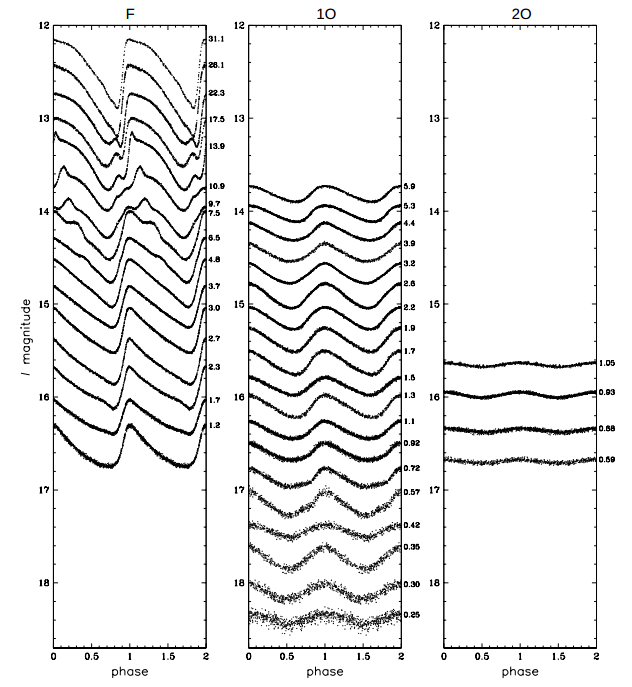
\includegraphics[width = \textwidth]{./img/C2Datos/tiposCefeidas.png}
  \caption{Curvas de luz ilustrativas de Cefeidas en modo fundamental (izquierda), primer sobretono (mitad), segundo sobretono (derecha). Los números pequeños a la derecha de cada recuadro muestran los periodos redondeados de las curvas de luz presentadas en los recuadros. Tomado de \cite{soszynski_optical_2011}}
  \label{fig:tiposCefeidas}
\end{figure}

En el Catálogo de Estrellas Variables de OGLE-III, cada curva de luz está disponible en un archivo que contiene tres columnas con los valores de magnitud, fecha juliana \footnote{La fecha Juliana es el tiempo medido en días desde el 1 de enero de 4713 a. C.} en la que fue tomada cada medida y error en la medida de la magnitud. El número de medidas para cada objeto y la separación temporal varía ampliamente. La separación mínima dos mediciones en toda la muestra es de 0.00147d, la máxima es 2156.9d y en promedio están separadas por 5.1d; por su parte el número promedio de observaciones por objeto es 759; el máximo, 5173; y el mínimo,  11. El 75\% de los objetos cuenta con más de 386 observaciones. Para todos los objetos estas observaciones están repartidas en los (número de años) años en que estuvo activo OGLE-III. En la figura \ref{fig:curvaDeLuz} se puede observar una curva de luz del catálogo de estrellas variables de OGLE-III.    


\begin{figure}
  \centering
  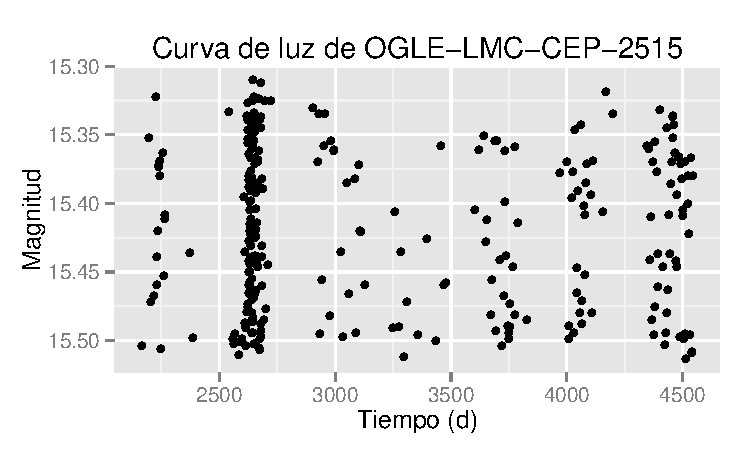
\includegraphics[width = 0.8\textwidth]{./img/C2Datos/curvaDeLuz.pdf}
  \caption{ Curva de luz de OGLE-LMC-CEP-2515 del catálogo OGLE-III. Los periodos en los que no hay mediciones corresponden a los momentos del año en los que la zona en la que se encuentra el objeto no puede ser observada debido a la posición relativa entre el Sol y la Tierra.}
  \label{fig:curvaDeLuz}
\end{figure}



\section{Características Seleccionadas \label{sec:atributos}}

Para una curva de luz denotaremos con $(m_{i})_{1\leq i\leq n}$, $(t_{i})_{1\leq i\leq n}$ y $j$ a su serie de magnitudes, tiempos y tipo de variabilidad respectivamente.

Idealmente, el vector de características debe ser fácil de cálcular y debe capturar las diferencias entre los tipos de variabilidad estelar. En la literatura \cite{debosscher_automated_2007, sarro_automated_2009, richards_machine-learned_2011} se han utilizado coeficientes de Fourier para este propósito. Suponiendo que los pares $(t_i,m_i)$ provienen de una versión corrupta  de la magnitud verdadera es posible encontrar estimadores de mpinimos cuadrados para los coeficientes con el periodograma de Lomb-Scargle. Sea $m(t)$ la magnitud verdadera de la estrella observada, $y(t) = m(t)+\epsilon$ la medición que es una versión corrupta de $m(t)$ con $\epsilon$ siendo una variable aleatoria. Los autores de \cite{debosscher_automated_2007} encuentran los parámetros $a_{ls}$, $f_l$ y $b_{ij}$ que mejor se ajustan a los datos de forma tal que $y$ es estimada por $\tilde{y}$
\begin{equation*}
\tilde{y}(t)=\sum_{l=1}^{3}\sum_{s=1}^{4}(a_{ls}\sen{2\pi f_l st} + b_{ls}\cos{2\pi f_l st}) + b_0
\end{equation*} 
% y utilizan una descripción de la curva en términos de las fases y $PH_{ls}$ y las amplitudes $A_{ls}$
% \begin{equation*}
% \tilde{y}(t)=\sum_{l=1}^{3}\sum_{s=1}^{4}A_{ls}\sen{(2\pi f_l st + PH_{ls})}  + b_0.
% \end{equation*} 
% A partir de $PH_{ls}$ es posible definir $PH''_{ls}$ que sea independiente de traslaciones temporales. 
Luego los autores utilizan estos coeficientes para dar una descripción de $y(t)$ que es independiente de traslaciones temporales. Lo importante no es entrear en los detalles de esta elección de parámetros sino resaltar que la búsqueda de estos es computacionalmente intensiva. Los autores de \cite{debosscher_automated_2007} utilizan el periodograma de Lomb-Scargle \cite{scargle_studies_1982} con el cual se obtiene una potencia para cada periodo posible. Predefinir los periodos posibles es un reto si no se tiene más información que la curva de luz de un objeto. Por ejemplo para clasificar las curvas de luz de Cefeidas Clásicas para el catálogo de OGLE-III \cite{soszynski_optical_2008-1} los autores probaron frecuencias entre 0.0 y 24.0 ciclos por día en aumentos de frecuencias de 0.0001 para 32 millones de objetos, para lo cual utilizaron supercomputadores del  \textit{Centre for Mathematical and Computational Modeling} de la Universidad de Varsovia, siguido de un análisis que llevó a la inspección manual de decenas de miles de curvas de luz. En este trabajo, basado en los hallazgos de \cite{rodriguez_feliciano_alisis_2012} y \cite{sabogal_search_2014}, proponemos utilizar en lugar de estos coeficientes, variables descriptivas de la serie de magnitudes (ver tabla \ref{cuadro:variablesUtilizadas}) que pueden ser calculadas en tiempos abrumadoramente menores, con menos poder computacional y sin intervención manual.

\begin{table}[ht]
  \centering
  \begin{tabular}{rr}
    \hline
    Cantidad & Fórmula  \\
    \hline
    Media& $\mu =\frac{1}{n}\sum_{i} m_{i}$ \\ 
    Desviación estándar& $\sigma = \sqrt{\frac{1}{n}\sum_{i} (m_{i}-\mu)^{2}}$ \\
    Sesgo & $\frac{1}{n}\sum_{i}{\left(\frac{m_{i}-\mu}{\sigma}\right)^{3}}$ \\
    Curtosis& $\frac{1}{n}\sum_{i}{\left(\frac{m_{i}-\mu}{\sigma}\right)^{4}}$ \\
    Rango& $\max_{i}m_{i} - \min_{i}m_{i}$ \\
    Variación cuadrática& $\frac{1}{n}\sum_{i}(m_{i}-m_{i-1})^{2}$ \\
    Valor Abbe \cite{mowlavi_searching_2014}& $\mathcal{A}=\frac{n}{2(n-1)}\frac{\sum_{i}{(m_{i}-m_{i-1})^{2}}}{\sum_{i}{(m_{i}-\mu})^2}$ \\
    Abbe promedio \cite{mowlavi_searching_2014}& $\bar{\mathcal{A}_{t}}$ \\
    Entropía de Shannon \cite{shannon_mathematical_1948} & $\sum_{i}{-p_{i}\log_{2}{p_{i}}}$ \\
    Entropía de Rényi\cite{renyi_measures_1961}& $\frac{1}{1-\alpha}\log_{2}{\sum_{x}p_{i}^{\alpha}}$\\
    \hline
  \end{tabular}
  \caption{Variables utilizadas}
  \label{cuadro:variablesUtilizadas}
\end{table}

Bajo este punto de vista, las magnitudes son vistas como una variable aleatoria independiente del tiempo y las cantidades de la tabla \ref{cuadro:variablesUtilizadas} son variables descriptivas de su densidad. En la figura \ref{fig:curvaHist} se observa una curva de luz y la densidad estimada de sus magnitudes. Al utilizar la distribución de la serie de magnitudes se asume que el número de observaciones es lo suficientemente grande, que estas son hechas en intervalos que evitan el aliasing y que son hechas durante más de un periodo del objeto observado. Es de esperar que las curvas que tienen formas similares, es decir, que pertenecen al mismo tipo de variabilidad estelar, tengan densidades de magnitudes similares y que, por ende, los parámetros descriptivos utilizados también sean similares.


\begin{figure}
  \centering
  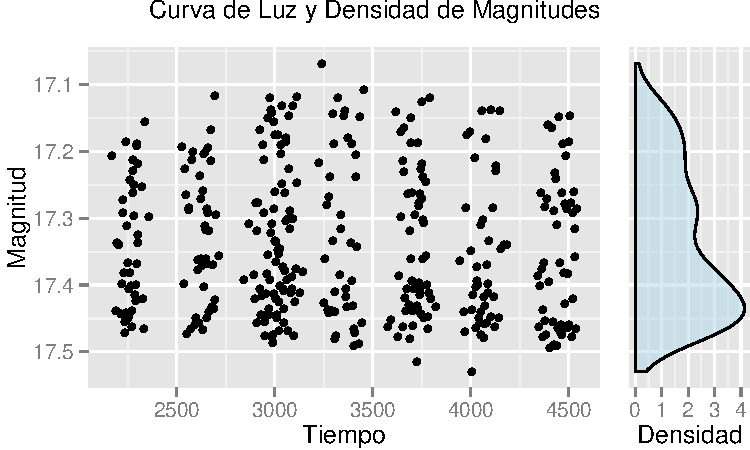
\includegraphics[width = 0.8\textwidth]{./img/CClasificacion/curvaHist.pdf}
  \caption{Curva de luz OGLE-LMC-CEP-0503 y densidad estimada de las magnitudes. }
  \label{fig:curvaHist}
  \centering
\end{figure}

La media $\mu$ y la desviación estándar $\sigma$ (ver cuadro \ref{cuadro:variablesUtilizadas}) son variables descriptivas bien conocidas. En este caso la media es el valor al rededor del cual la serie de magnitudes oscila y la desviación una medida de la amplitud de estas oscilaciones. (Dar argumentos astronómicos). La figura \ref{fig:mediaDesv} muestra la densidad de cada una de las clases en el plano $\mu$-$\sigma$. Aunque las diferentes clases se superponen en este plano, hay pares de clases que pueden ser distinguidas como $\delta$Sct y RRLyr.

\begin{figure}
  \centering
  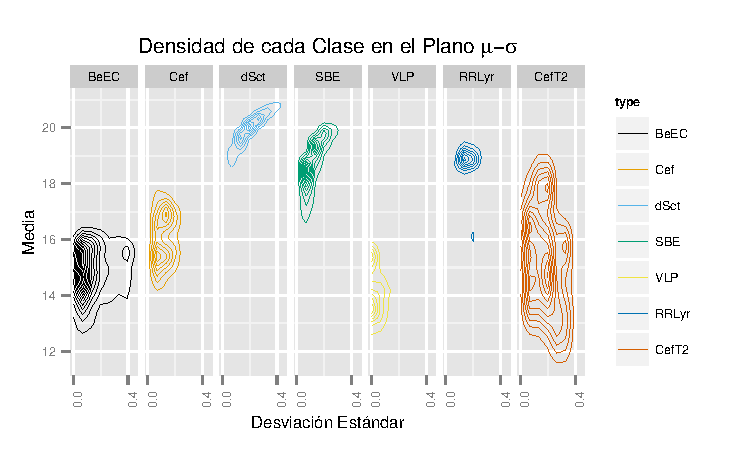
\includegraphics[width = \textwidth]{./img/CClasificacion/mediaDesv.pdf}
  \caption{}
  \label{fig:mediaDesv}
  \centering
\end{figure}

Basado en el trabajo de \cite{rodriguez_feliciano_alisis_2012} utilizamos el sesgo y la curtosis como características. El sesgo es el tercer momento central estandarizado \footnote{El k-ésimo momento centrado de una variable aleatoria $X$ (o de su distribución) es $\mu_{k} =E[(X-\mu)^{k}]$, siendo $\mu$ su media. Su k-ésimo momento central estandarizado es $\frac{\mu_k}{\sigma^k}$, siendo $\sigma$ la desviación estándar.} y es una medida de de la asimetría de una distribución. Una distribución es simétrica si su sesgo es $0$, su cola izquierda es más larga si su sesgo es positivo y su cola derecha es más larga si su sesgo es negativo. Por su parte la curtosis es el cuarto momento central estndarizado. Es una medida de qué tan concentrada está la distribución al rededor de la media. La curtosis de una distribución normal es $3$ y con frecuencia se estudia una cantidad llamada exceso de curtosis que es el resultado de restarle $3$ a la curtosis. Los autores de \cite{rodriguez_feliciano_alisis_2012}  encontraron que algunos tipos de variabilidad estelar podían ser distinguidos utilizando clasificadores lineales en el plano sesgo-curtosis.

Dado que la estimación de el sesgo y la curtosis con las fórmulas del cuadro \ref{cuadro:variablesUtilizadas} requiere de calcular las potencias $(\mu-m_i)^3$ y $(\mu-m_i)^4$, son propensas a dar estimaciones erróneas en el caso de que existan datos atípicos. Calculamos también la l-curtosis y el l-sesgo\footnote{Los l-momentos son combinaciones lineales de los estadísticos de orden. Son robustos, toman valores entre 0 y 1, y la interpretación de sus valores es análoga a la de los momentos. De la misma manera en que se define el sesgo y la curtosis muestral, es posible definir la l-curtosis y el l-sesgo. Fuero propuestos en (cita l-momentos) y su cálculo fue realizado utilizando el paquete lmoments(cita paquete l-moments) para R} y reemplazando el sesgo y la curtosis por estas cantidades no encontramos dierencias importantes en el poder para clasificar de los clasificadores que utlizamos. Esto puede ser un indicador de que no existe una proporción grande de datos atípicos en las curvas de luz. Por su simplicidad utilizamos el sesgo y la curtosis.  


\section{Clasificación}
\subsection{k Vecinos Más Cercanos}
\begin{table}[ht]
  \centering
  \caption{k = 1} 
  \label{table:cmknn}
  \begin{tabular}{rrrrrrrr}
    \hline
    & becand & cep & dcst & ebs & lpv & rrlyr & t2cep \\ 
    \hline
    becand & 381 &   1 &   0 &  50 &  41 &   0 &   0 \\ 
    cep &   1 & 6595 &   4 & 172 &  54 & 986 &  87 \\ 
    dcst &   0 &   7 & 2064 & 340 &  13 & 151 &   0 \\ 
    ebs &  51 & 184 & 536 & 30129 & 573 & 668 &  29 \\ 
    lpv &  42 & 187 &  19 & 944 & 342740 & 371 & 158 \\ 
    rrlyr &   0 & 971 & 165 & 595 & 308 & 41911 & 217 \\ 
    t2cep &   0 &  59 &   0 &  29 &  53 & 130 & 112 \\ 
    \hline
  \end{tabular}
\end{table}

\begin{table}[ht]
  \centering
  \caption{k=1, validación cruzada de 10 iteraciones} 
  \label{table:cmCvKnn}
  \begin{tabular}{rrrrrrrr}
    \hline
    & becand & cep & dcst & ebs & lpv & rrlyr & t2cep \\ 
    \hline
    becand & 0.80 & 0.00 & 0.00 & 0.00 & 0.00 & 0.00 & 0.00 \\ 
    cep & 0.00 & 0.82 & 0.00 & 0.01 & 0.00 & 0.02 & 0.14 \\ 
    dcst & 0.00 & 0.00 & 0.74 & 0.01 & 0.00 & 0.00 & 0.00 \\ 
    ebs & 0.11 & 0.02 & 0.19 & 0.93 & 0.00 & 0.02 & 0.05 \\ 
    lpv & 0.09 & 0.02 & 0.01 & 0.03 & 1.00 & 0.01 & 0.26 \\ 
    rrlyr & 0.00 & 0.12 & 0.06 & 0.02 & 0.00 & 0.95 & 0.36 \\ 
    t2cep & 0.00 & 0.01 & 0.00 & 0.00 & 0.00 & 0.00 & 0.19 \\ 
    \hline
  \end{tabular}
\end{table}
\subsection{Máquinas de Soporte Vectorial}

\begin{table}[ht]
  \centering
  \caption{$\gamma = 0.1$, costo = $16$} 
  \label{table:cmSvm}
  \begin{tabular}{rrrrrrrr}
    \hline
    & becand & cep & dcst & ebs & lpv & rrlyr & t2cep \\ 
    \hline
    becand & 297 &   0 &   2 &  26 &  16 &   0 &   0 \\ 
    cep &   0 & 4622 &   0 &  55 &  85 & 788 &  69 \\ 
    dcst &   0 &   0 & 1683 & 163 &   4 &  47 &   0 \\ 
    ebs &  89 &  48 & 865 & 29439 & 198 & 563 &   5 \\ 
    lpv &  89 & 490 &  22 & 1380 & 342823 & 1113 & 255 \\ 
    rrlyr &   0 & 2844 & 216 & 1196 & 656 & 41706 & 274 \\ 
    t2cep &   0 &   0 &   0 &   0 &   0 &   0 &   0 \\ 
    \hline
  \end{tabular}
\end{table}

\begin{table}[ht]
  \centering
  \caption{$\gamma = 0.1$, costo = $16$, validación cruzada de 10 iteraciones} 
  \label{table:cmCvSvm}
  \begin{tabular}{rrrrrrrr}
    \hline
    & becand & cep & dcst & ebs & lpv & rrlyr & t2cep \\ 
    \hline
    becand & 0.63 & 0.00 & 0.00 & 0.00 & 0.00 & 0.00 & 0.00 \\ 
    cep & 0.00 & 0.58 & 0.00 & 0.00 & 0.00 & 0.02 & 0.11 \\ 
    dcst & 0.00 & 0.00 & 0.60 & 0.01 & 0.00 & 0.00 & 0.00 \\ 
    ebs & 0.19 & 0.01 & 0.31 & 0.91 & 0.00 & 0.01 & 0.01 \\ 
    lpv & 0.19 & 0.06 & 0.01 & 0.04 & 1.00 & 0.03 & 0.42 \\ 
    rrlyr & 0.00 & 0.36 & 0.08 & 0.04 & 0.00 & 0.94 & 0.45 \\ 
    t2cep & 0.00 & 0.00 & 0.00 & 0.00 & 0.00 & 0.00 & 0.00 \\ 
    \hline
  \end{tabular}
\end{table}

\subsection{Árboles de Clasificación y Regresión}
% Matriz de confusión para Cart
\begin{table}[ht]
  \centering
  \caption{Matriz de confusión para CART} 
  \label{cuadro:cmCart}
  \begin{tabular}{rrrrrrrr}
    \hline
    & becand & cep & dcst & ebs & lpv & rrlyr & t2cep \\ 
    \hline
    becand & 470 &  12 &   6 & 1039 & 8906 &  47 &  18 \\ 
    cep &   0 & 6210 &  12 &  18 & 320 & 3098 &  92 \\ 
    dcst &   0 &  35 & 2511 & 5538 &  91 & 1615 &   1 \\ 
    ebs &   0 &   1 & 148 & 21346 & 346 &  64 &   1 \\ 
    lpv &   5 & 107 &  24 & 1762 & 304810 & 100 &   3 \\ 
    rrlyr &   0 & 648 &  82 & 552 & 13880 & 34313 &  92 \\ 
    t2cep &   0 & 991 &   5 & 2004 & 15429 & 4980 & 396 \\ 
    \hline
  \end{tabular}
\end{table}

% Errores de validación cruzada para cart
\begin{table}[ht]
  \centering
  \caption{Tasas de clasificación estimadas por validación cruzada de 10 iteraciones} 
  \label{table:cmCvCart}
  \begin{tabular}{rrrrrrrr}
    \hline
    & becand & cep & dcst & ebs & lpv & rrlyr & t2cep \\ 
    \hline
    becand & 0.99 & 0.00 & 0.00 & 0.03 & 0.03 & 0.00 & 0.03 \\ 
    cep & 0.00 & 0.78 & 0.00 & 0.00 & 0.00 & 0.07 & 0.15 \\ 
    dcst & 0.00 & 0.00 & 0.90 & 0.17 & 0.00 & 0.04 & 0.00 \\ 
    ebs & 0.00 & 0.00 & 0.05 & 0.66 & 0.00 & 0.00 & 0.00 \\ 
    lpv & 0.01 & 0.01 & 0.01 & 0.05 & 0.89 & 0.00 & 0.00 \\ 
    rrlyr & 0.00 & 0.08 & 0.03 & 0.02 & 0.04 & 0.78 & 0.15 \\ 
    t2cep & 0.00 & 0.12 & 0.00 & 0.06 & 0.04 & 0.11 & 0.66 \\ 
    \hline
  \end{tabular}
\end{table}


\subsection{Bosques Aleatorios}


% \begin{appendices}

%   \chapter{El Problema de Aprendizaje} %\label{sec:problemaAprendizaje}}

%   \chapter{K Vecinos Más cercanos}

%   \chapter{Árboles de Clasificación y Regresión}

%   \chapter{Máquinas de Soporte Vectorial}
  
%   \chapter{Bosques Aleatorios}
  
% \end{appendices}

%\chapter{Cosas que la evolución se llevó}

%\section{vieja introducción}
% En este trabajo abordamos el problema de clasificar curvas de luz de estrellas variables por su tipo de variabilidad \footnote{Las estrellas variables son estrellas cuya magnitud cambia en el tiempo (ver nota \ref{nota:curvasDeLuz}). Pueden ser periódicas o no periódicas y se pueden clasificar como pulsantes, eruptivas o variables eclipsantes aunque existen subclases de variabilidad estelar. Una estrella puede ser clasificada en estas subclases conociendo su curva de luz (ver el capítulo 13 de \cite{karttunen_fundamental_2007}).} como un problema de aprendizaje supervisado. Para esto utilizamos una parte de los resultados de la tercera fase del \textit{Optical Gravitational Lensing Experiment} (OGLE III) que contiene curvas de luz  de estrellas previamente clasificadas en seis tipos de variabilidad estelar y curvas de luz de estrellas candidatas a ser clasificadas como Be (ver capítulo \ref{cap:losDatos}) (ver cuadro \ref{cuadro:datosUsados}). 


% Para abordar el problema de clasificación adoptamos el siguiente punto de vista. Cada curva de luz $c_i = \{(t_{n}^{i}, m_{n}^{i})\}_{n}$ es una sucesión de parejas donde la primera es el tiempo y la segunda es la magnitud medida en ese instante.  Debido a limitaciones en el tiempo de observación, fallas técnicas, periodos de matenimiento de los instrumentos utilizados y el hecho de que no todas las regiones del cielo son observables durante todo el año y solo se puede observar una región limitada en cada oportunidad, las curvas de luz no constan del mismo número de observaciones y éstas no son hechas en intervalos regulares ($t_{k} - t_{k+1}$ no es constante). Una forma de hacer frente a esto es asignarle a cada curva de luz $c_i$ un vector de atributos $\vec{x_{i}} = \vec{x_{i}}(c_i)\in\mathbb{R}^{n}$ calculados a partir de de $c_i$ (ver sección \ref{sec:atributos}) que intenten describir los tipos de variabilidad. Como los elementos de la muestra han sido clasificados previamente, le asignamos a cada curva de luz $c_i$ una etiqueta $j_i\in J=\{\text{RR Lyr}, \dots, \text{BeSC}\}$ (ver tabla \ref{cuadro:datosUsados}) que corresponde al tipo de variabilidad estelar de la estrella observada.  Dicha etiqueta, a su vez, es heredada por el vector de atributos $\vec{x}_i$.

% Si nuestra elección de atributos es acertada, podremos utilizar la representación de las curvas de luz en el espacio de atributos para realizar la clasificación, esto es, existirá una función $g:\mathbb{R}^n\rightarrow J$ que, de alcanzar la mejor tasa de clasificación correcta posible para esos atributos, le asigna a cada curva de luz el tipo de variabilidad correcto con probabilidad alta (ver capítulo \ref{cap:problemaAprendizaje}). Puede suceder que, si los atributos no caracterizan los diferentes tipos de variabilidad, incluso utilizando el mejor clasificador posible (la mejor función $g$) no sea posible alcanzar errores de clasificación bajos. De esto se sigue que la elección de atributos es crucial para lograr una buena clasificación. La elección de los atributos utilizados se discute en la sección \ref{sec:atributos}.

% El siguiente problema será el de inferir (aprender) de los datos una función $\hat{g}:\mathbb{R}^n\rightarrow J$ que se aproxime tanto como sea posible a la mejor regla posible en cuanto a que maximice la probabilidad de clasificación correcta. Para encontrar esta regla existen diferentes aproximaciones y algorítmos que permiten la división del espacio de atributos en zonas a cada una de las cuales se le asigna un tipo de variabilidad. En la práctica no se conoce la mejor regla posible porque esto requeriría el conocimiento de la distribución exacta de los atributos (ver capítulo \ref{cap:problemaAprendizaje}). Tampoco se conoce el mínimo error de clasificación posible por lo que, para la selección del mejor clasificador entre los posibles, se utilizan estimaciones del error de clasificación que utilizan la muestra disponible, en este caso validación cruzada (ver sección \ref{sec:estimacionError}).En el capítulo \ref{cap:aprendizaje} utilizamos k vecinos más cercanos, arboles de clasificación y regresión; y maquinas de soporte vectorial para inferir la función $\hat{g}$. Asímismo analizamos los estimados de la probabilidad de error al usar cada algorítmo y comentamos las ventajas comparativas de cada uno. Estos tres métodos son muy diferentes en su naturaleza, fueron elegidos porque han mostrado ser efectivos en gran variedad de aplicaciones y por su carácter no paramétrico y no lineal. 

% Así la clasificación de una curva de luz correspondiente a una estrella cuyo tipo de variabilidad es desconocido será un proceso de dos pasos. El primero será la extracción de los atributos. El segundo paso será la clasificación basada en los atributos utilizando la función $\hat{g}$ que fue encontrada con ayuda de la muestra disponible. Esta clasificación será correcta con cierta probabilidad, estimada con validación cruzada.

% Este documento está organizado de la siguiente manera. En el capítulo \ref{cap:losDatos} damos un análisis descriptivo del conjunto de datos que consideramos y discutimos la elección de los atributos para realizar la clasificación. En el capítulo \ref{cap:problemaAprendizaje} discutimos brevemente el problema de clasificación en general, describimos el mejor clasificador posible (el clasificador de Bayes), discutimos la imposibilidad de utilizarlo en la mayoría de aplicaciones complejas y describimos el método que usamos para estimar la probabilidad de error de los clasificadores. En el capítulo \ref{cap:aprendizaje} describimos los métodos de clasificación utilizados, damos los estimados del error de clasificación y comparamos los resultados con otros valores dados en la literatura.

\bibliographystyle{plain}
\bibliography{tesisMatematicas}

\end{document}
